\documentclass[preprint,12pt]{elsarticle}
%\documentclass[final,5p,times,twocolumn]{elsarticle}

\usepackage{amsmath,amssymb,amsfonts}
\usepackage{graphicx}
\usepackage{booktabs}
\setlength{\abovetopsep}{4pt}
\usepackage{array}
\usepackage{multirow}
\usepackage{xcolor}
\usepackage{url}
\usepackage[hidelinks]{hyperref}
\usepackage{tikz}
\usetikzlibrary{arrows.meta, positioning, fit, backgrounds, calc, shapes.geometric, decorations.pathreplacing}

% Figure palette (Okabe--Ito, colour-blind safe). One colour per evidence
% channel, used identically in every figure.
\definecolor{cText}{HTML}{0072B2}      % text passages, dense retrieval
\definecolor{cGraph}{HTML}{009E73}     % knowledge graph
\definecolor{cVis}{HTML}{E69F00}       % figures and crops
\definecolor{cGen}{HTML}{CC79A7}       % generator
\definecolor{cCtrl}{HTML}{7F7F7F}      % evidence controls
\definecolor{cAlt}{HTML}{F0E442}       % non-graph comparators
\definecolor{cCredit}{HTML}{0072B2}    % state: credited to gold evidence
\definecolor{cNotCredit}{HTML}{E69F00} % state: correct, not credited
\definecolor{cErr}{HTML}{D55E00}       % state: error
\tikzset{
  box/.style = {draw=black!65, rounded corners=1.5pt, align=center,
                line width=0.45pt, inner sep=2.5pt, font=\scriptsize,
                minimum height=6mm,
                execute at begin node={\hyphenpenalty=10000}},
  arr/.style = {-{Latex[length=1.5mm,width=1.2mm]}, line width=0.45pt,
                draw=black!70},
  lab/.style = {font=\scriptsize\itshape, text=black!70, inner sep=1.5pt},
  sub/.style = {font=\scriptsize, text=black!75},
}

% -------------------------------------------------------------------------
% Revision draft (2026-10-20). Rewritten from the version desk-rejected by
% Information Processing & Management (IPM-D-26-06642, 2026-09-02); that
% version is kept as manuscript_v1_rejected_IPM.tex.
%
% Everything that depends on the new paid runs is a red \tbd{} placeholder.
% Grey "Writer note" boxes say how to read each comparison under either
% outcome. Set \draftnotesfalse to hide the notes; no \tbd may remain in the
% submitted version.
% -------------------------------------------------------------------------
\newif\ifdraftnotes
\draftnotestrue
\newcommand{\tbd}[1]{\textcolor{red}{[#1]}}
\newcommand{\note}[1]{\ifdraftnotes\par\smallskip\noindent\fcolorbox{black!40}{black!4}{\parbox{\dimexpr\linewidth-2\fboxsep-2\fboxrule}{\footnotesize\textbf{Writer note.} #1}}\par\smallskip\fi}

% Target order agreed 2026-09-03: Data & Knowledge Engineering, then Applied
% Artificial Intelligence. (Knowledge-Based Systems first is a proposal, not
% yet agreed.)
\journal{Data \& Knowledge Engineering}

\begin{document}
\begin{frontmatter}

\title{A Controlled Evaluation of Evidence Attribution in Graph-Augmented and Multimodal RAG for Document Question Answering}

% \author[aff1]{Sokipriala Jonah\corref{cor1}}
% \ead{jonahs@uni.coventry.ac.uk}
% \author[aff1]{Opeoluwa Akinseloyin}
% \author[aff1]{Michael Ajao-Olarinoye}
% \author[aff1]{Abiola Babatunde}
% \cortext[cor1]{Corresponding author}
% \affiliation[aff1]{
%     organization={Centre for Computational Science and Mathematical Modelling,
%     Coventry University},
%     city={Coventry},
%     country={United Kingdom}
% }

\begin{abstract}
When a retrieval-augmented generation (RAG) system answers correctly, the
answer may come from the gold passage, from another passage, from the model's
own knowledge, or from a caption that restates a figure. Accuracy alone cannot
separate these routes, so augmentation gains may reflect more context, easier
questions, or prior exposure. We define eight evidence states that assign each
outcome to one route, using gold provenance, a closed-book arm, and a
model-judged sufficiency check, and we split any accuracy difference into an
evidence-access and an evidence-use term. For graphs, an LLM-extracted
knowledge graph either adds triples to the prompt or expands the candidate
set, and the expansion is compared at equal budget with five non-graph
retrievers and HippoRAG\,2 on 200 human-authored HotpotQA questions with five
generators. For figures, CLIP retrieval is evaluated with four generators on 150
human-authored SPIQA questions screened for caption leakage. At equal budget the graph
expansion does not beat dense top-5 retrieval on bridge questions in exact
match or judge accuracy (both $+0.004$; judge 95\% CI $-0.034$ to $+0.044$),
consistent with a budget effect. HippoRAG\,2 raises judge accuracy on bridge
questions by 0.160, mostly through the access term, but not on comparison
questions. Fewer than half of the correct HotpotQA answers can be credited to
retrieved gold evidence, even when both gold articles are supplied. On figure
questions the top-ranked crop raises judge accuracy over text-only retrieval by
0.073 (95\% CI 0.038 to 0.110), and by 0.062 after text-recoverable and
closed-book-recoverable items are removed. Contrary to our prediction, the gain
is not larger on caption-flagged items. CLIP ranks the gold crop first for only
17\% of these questions, and supplying that crop raises accuracy by 0.358.
Accuracy alone would hide both the answers a generator can give without
evidence and the gain lost before evidence reaches it.

\end{abstract}

\begin{keyword}
Retrieval-augmented generation \sep
Evidence attribution \sep
Knowledge graphs \sep
Multimodal retrieval \sep
Evaluation methodology \sep
Document question answering
\end{keyword}
\end{frontmatter}

% =========================================================================
\section{Introduction}
\label{sec:intro}
% =========================================================================

Retrieval-augmented generation (RAG) conditions a language model on passages
retrieved at inference time~\cite{lewis2020rag,gao2023survey}. Two extensions
are now common in document question answering. Graph-based RAG extracts
entities and relations so that evidence spread across passages or documents
can be connected~\cite{edge2024graphrag,hipporag,guo2024lightrag}. Multimodal
RAG retrieves figures, tables, or page images and passes them to a
vision--language model~\cite{faysse2024colpali,cho2024m3docrag,dong2025mmdocrag}.
Both are usually evaluated end to end, by running a configuration on a
question set and comparing its accuracy with a text-only baseline.

That comparison answers whether the configuration scored higher. It does not
answer why. A graph-augmented retriever that returns five passages instead of
three may win because of the graph or because of the two extra passages. A
multimodal system may win on figure questions whose answers also appear in the
caption. On public corpora such as Wikipedia or arXiv, a generator may answer
correctly without any retrieved gold evidence, because it saw the source during
pretraining~\cite{roberts2020knowledge,mallen2023popqa,kandpal2023longtail}.
Each of these routes produces a correct answer, and accuracy counts them
identically.

Our earlier study of the same systems~\cite{jonah2026whendo} illustrates the
problem. Graph expansion at the retrieval stage raised gold-evidence
completeness on 50 HotpotQA bridge questions from 0.22 to 0.46 and improved
accuracy for all four generators. But the expanded system received up to five
passages against the baseline's three. The strongest cross-document result came
from questions that had been generated from the same graph the retriever then
searched. And generators answered 35--71\% of incomplete-evidence questions
correctly on public corpora, compared with none on an obscure one. None of these
observations invalidates the result, but none can be resolved by accuracy
alone. The present study draws a new sample of 100 bridge and 100 comparison
questions and pools its corpus from 600 HotpotQA questions rather than 300,
so its completeness figures are not directly comparable with the earlier
ones. The present paper revises that study. It keeps the graph and
multimodal systems and the SPIQA and PubLayNet corpora, and adds the evidence
states and the access and use split, equal-budget non-graph arms and
HippoRAG\,2, closed-book, shuffled, oracle, and partial-gold arms, a
caption-leakage screen on questions written by SPIQA's annotators, five
current generators, and pre-specified paired tests.

This paper treats the question of where a correct answer came from as the
primary object of evaluation, and makes three contributions. The first is a
set of eight operational evidence states that assign each
question--system--generator outcome to one evidence route
(Section~\ref{sec:framework}). The states are computed from gold provenance,
a closed-book arm, and a model-judged sufficiency check. Any accuracy
difference between two systems then splits exactly into an \emph{access}
term, for changes in which evidence the generator saw, and a \emph{use} term,
for changes in how well it answered with evidence of the same completeness.

The second contribution is a controlled test of graph augmentation. The same
extracted graph is applied at the generation stage (+KG) and at the retrieval
stage (+KGret), and +KGret is compared at an equal candidate budget with
dense, BM25, reciprocal-rank-fusion, lexical entity-expansion, and
random-padding retrieval and with HippoRAG\,2~\cite{gutierrez2025hipporag2}.
The questions are written by HotpotQA's annotators and scored against their
references with the benchmark's exact match and F1, with answer containment,
and by a judge (Section~\ref{sec:res-graph}).
The third is a leakage-aware test of multimodal augmentation, in which figure
questions written by SPIQA's annotators~\cite{spiqa} are screened for caption
leakage and the multimodal gain is re-estimated after flagged and
closed-book-recoverable items are removed, while an oracle-image arm separates
retrieval failure from figure-reading failure (Section~\ref{sec:res-mm}).

All research questions, hypotheses, primary outcomes, and statistical tests
were fixed before any results were collected (Section~\ref{sec:rqs}), and
every later change to that plan is listed with its reason in
Table~\ref{tab:deviations}.
Figure~\ref{fig:design} summarises what each graph and control arm supplies
to the generator.

% Study design: what each arm places in the generator's context. Rows share
% one column grid so that only the candidate set (and, for +KG, the prompt
% extras) changes between rows.
\begin{figure*}[t]
\centering
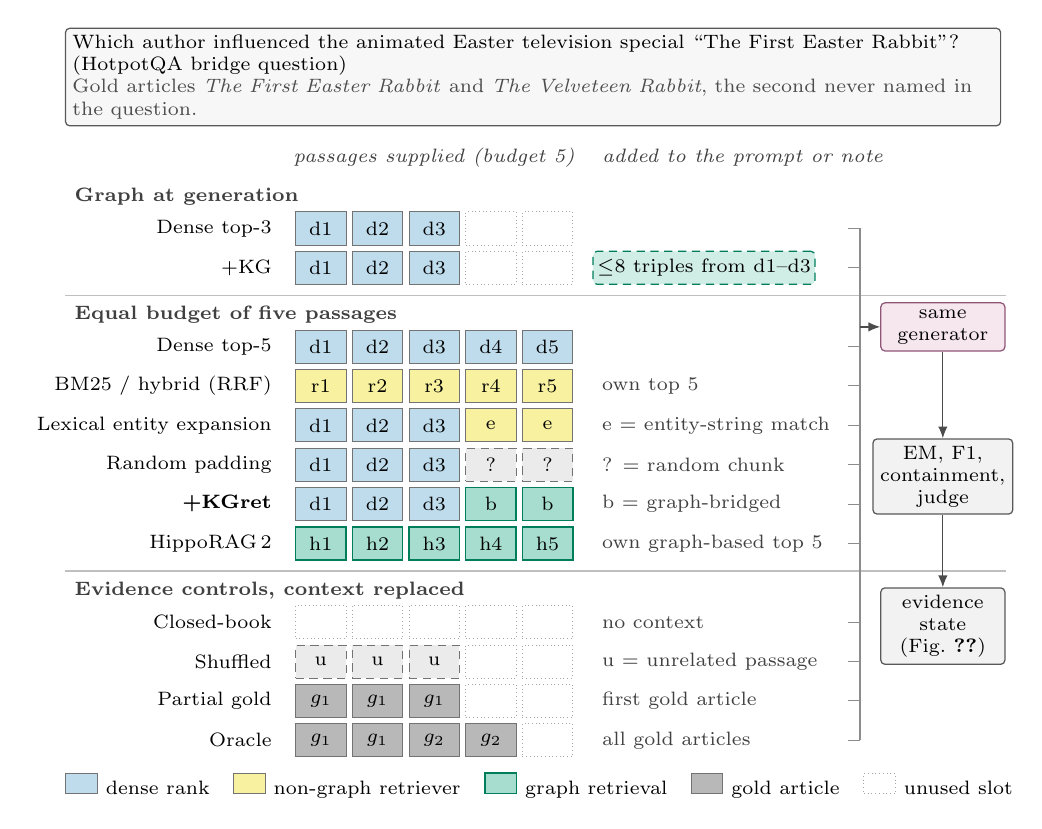
\begin{tikzpicture}[
  slot/.style  = {draw=black!55, line width=0.35pt, minimum width=6.4mm,
                  minimum height=4.2mm, inner sep=0pt, font=\scriptsize},
  dense/.style = {slot, fill=cText!25},
  alt/.style   = {slot, fill=cAlt!50},
  rnd/.style   = {slot, fill=black!8, densely dashed},
  grf/.style   = {slot, fill=cGraph!35, draw=cGraph!80!black, line width=0.55pt},
  gold/.style  = {slot, fill=black!28},
  empty/.style = {slot, draw=black!35, densely dotted},
  rowlab/.style= {font=\scriptsize, anchor=east, align=right},
  grp/.style   = {font=\scriptsize\bfseries, anchor=west, text=black!75},
  xtra/.style  = {font=\scriptsize, anchor=west, align=left, text=black!75},
]
\def\sx{3.15}  % x of slot 1
\def\sw{0.72}  % slot pitch
\def\xx{6.6}   % x of the prompt-extras column
\newcommand{\slots}[6]{%
  \foreach \st/\tx [count=\i from 0] in {#2,#3,#4,#5,#6}
    \node[\st] at (\sx+\i*\sw,#1) {\tx};}

% Example question
\node[box, fill=black!3, text width=117mm, align=left, anchor=north west]
  at (-0.1,1.95) {Which author influenced the animated Easter television
  special ``The First Easter Rabbit''? (HotpotQA bridge question)\\
  \textcolor{black!70}{Gold articles \emph{The First Easter Rabbit} and
  \emph{The Velveteen Rabbit}, the second never named in the question.}};

% Column headers
\node[font=\scriptsize\itshape, text=black!75] at (\sx+2*\sw,0.3) {passages supplied (budget 5)};
\node[font=\scriptsize\itshape, text=black!75, anchor=west] at (\xx,0.3) {added to the prompt or note};

% --- Group 1: graph at the generation stage
\node[grp] at (-0.1,-0.2) {Graph at generation};
\node[rowlab] at (2.65,-0.6) {Dense top-3};
\slots{-0.6}{dense/d1}{dense/d2}{dense/d3}{empty/}{empty/}
\node[rowlab] at (2.65,-1.1) {+KG};
\slots{-1.1}{dense/d1}{dense/d2}{dense/d3}{empty/}{empty/}
\node[box, fill=cGraph!18, draw=cGraph!80!black, densely dashed, anchor=west,
      minimum height=4.2mm, inner sep=1.5pt] at (\xx,-1.1)
      {$\le$8 triples from d1--d3};

% --- Group 2: equal budget
\draw[black!25] (-0.1,-1.45) -- (11.85,-1.45);
\node[grp] at (-0.1,-1.7) {Equal budget of five passages};
\node[rowlab] at (2.65,-2.1) {Dense top-5};
\slots{-2.1}{dense/d1}{dense/d2}{dense/d3}{dense/d4}{dense/d5}
\node[rowlab] at (2.65,-2.6) {BM25 / hybrid (RRF)};
\slots{-2.6}{alt/r1}{alt/r2}{alt/r3}{alt/r4}{alt/r5}
\node[xtra] at (\xx,-2.6) {own top 5};
\node[rowlab] at (2.65,-3.1) {Lexical entity expansion};
\slots{-3.1}{dense/d1}{dense/d2}{dense/d3}{alt/e}{alt/e}
\node[xtra] at (\xx,-3.1) {e = entity-string match};
\node[rowlab] at (2.65,-3.6) {Random padding};
\slots{-3.6}{dense/d1}{dense/d2}{dense/d3}{rnd/?}{rnd/?}
\node[xtra] at (\xx,-3.6) {? = random chunk};
\node[rowlab] at (2.65,-4.1) {\textbf{+KGret}};
\slots{-4.1}{dense/d1}{dense/d2}{dense/d3}{grf/b}{grf/b}
\node[xtra] at (\xx,-4.1) {b = graph-bridged};
\node[rowlab] at (2.65,-4.6) {HippoRAG\,2};
\slots{-4.6}{grf/h1}{grf/h2}{grf/h3}{grf/h4}{grf/h5}
\node[xtra] at (\xx,-4.6) {own graph-based top 5};

% --- Group 3: evidence controls
\draw[black!25] (-0.1,-4.95) -- (11.85,-4.95);
\node[grp] at (-0.1,-5.2) {Evidence controls, context replaced};
\node[rowlab] at (2.65,-5.6) {Closed-book};
\slots{-5.6}{empty/}{empty/}{empty/}{empty/}{empty/}
\node[xtra] at (\xx,-5.6) {no context};
\node[rowlab] at (2.65,-6.1) {Shuffled};
\slots{-6.1}{rnd/u}{rnd/u}{rnd/u}{empty/}{empty/}
\node[xtra] at (\xx,-6.1) {u = unrelated passage};
\node[rowlab] at (2.65,-6.6) {Partial gold};
\slots{-6.6}{gold/$g_1$}{gold/$g_1$}{gold/$g_1$}{empty/}{empty/}
\node[xtra] at (\xx,-6.6) {first gold article};
\node[rowlab] at (2.65,-7.1) {Oracle};
\slots{-7.1}{gold/$g_1$}{gold/$g_1$}{gold/$g_2$}{gold/$g_2$}{empty/}
\node[xtra] at (\xx,-7.1) {all gold articles};

% Shared generator and scoring
\draw[black!45, line width=0.5pt] (10.0,-0.6) -- (10.0,-7.1);
\foreach \y in {-0.6,-1.1,-2.1,-2.6,-3.1,-3.6,-4.1,-4.6,-5.6,-6.1,-6.6,-7.1}
  \draw[black!45, line width=0.4pt] (9.85,\y) -- (10.0,\y);
\node[box, fill=cGen!18, draw=cGen!70!black, text width=14mm] (gen) at (11.05,-1.85)
  {same generator};
\node[box, fill=black!5, text width=16mm] (score) at (11.05,-3.75)
  {EM, F1,\\ containment,\\ judge};
\node[box, fill=black!5, text width=14mm] (state) at (11.05,-5.65)
  {evidence state (Fig.~\ref{fig:states})};
\draw[arr] (10.0,-1.85) -- (gen.west);
\draw[arr] (gen) -- (score);
\draw[arr] (score) -- (state);

% Legend
\node[anchor=north west, inner sep=0pt] at (-0.1,-7.5) {%
  \scriptsize
  \begin{tabular}{@{}l@{\hspace{1mm}}l@{\hspace{3mm}}l@{\hspace{1mm}}l@{\hspace{3mm}}l@{\hspace{1mm}}l@{\hspace{3mm}}l@{\hspace{1mm}}l@{\hspace{3mm}}l@{\hspace{1mm}}l@{}}
  \tikz\node[dense, minimum width=4mm, minimum height=2.6mm] {};& dense rank &
  \tikz\node[alt, minimum width=4mm, minimum height=2.6mm] {};& non-graph retriever &
  \tikz\node[grf, minimum width=4mm, minimum height=2.6mm] {};& graph retrieval &
  \tikz\node[gold, minimum width=4mm, minimum height=2.6mm] {};& gold article &
  \tikz\node[empty, minimum width=4mm, minimum height=2.6mm] {};& unused slot
  \end{tabular}};
\end{tikzpicture}
\caption{Passages each arm places in the generator's context for one HotpotQA
bridge question. All rows share the question, generator, and scoring. The
passage rows also share one prompt and differ only in the passages supplied
and, for +KG, in the triples added to it. The evidence controls replace the
context, and the closed-book arm uses a prompt that asks for the generator's
own knowledge.}
\label{fig:design}
\end{figure*}


% =========================================================================
\section{Related Work}
\label{sec:related}
% =========================================================================

\subsection{Graph-augmented retrieval}

GraphRAG builds an entity graph with an LLM and uses community summaries for
query-focused summarisation over a corpus~\cite{edge2024graphrag}. LightRAG
indexes entities and relations for lower-cost graph retrieval
\cite{guo2024lightrag}; RAPTOR builds a tree of recursive summaries
\cite{sarthi2024raptor}; Think-on-Graph, StructGPT, and KAPING condition the
generator on graph paths or retrieved triples
\cite{sun2024thinkongraph,jiang2023structgpt,baek2023kaping}; surveys
catalogue these designs~\cite{peng2024graphragsurvey}. HippoRAG applies
personalised PageRank over an OpenIE graph during retrieval
\cite{hipporag}, and HippoRAG\,2 adds passage nodes and query-to-triple
matching~\cite{gutierrez2025hipporag2}. These systems differ in where the graph
acts. Some change which passages are retrieved, while others only add
structured facts to the prompt. A controlled comparison of plain RAG and GraphRAG reports
that neither dominates and that the outcome depends on question type
\cite{ragvsgraphrag}. Our design isolates the stage variable by holding the
graph fixed and adds equal-budget non-graph expansions, which most graph-RAG
evaluations omit.

\subsection{Multimodal document RAG}

ColPali embeds page images directly~\cite{faysse2024colpali}; PixelRAG
retrieves and reads screenshots~\cite{wang2025pixelrag}; M3DocRAG and MMDocRAG
extend retrieval to multi-page and multi-document settings
\cite{cho2024m3docrag,dong2025mmdocrag}; benchmarks such as DocVQA, ChartQA,
and SPIQA evaluate question answering over document images, charts, and
scientific figures~\cite{mathew2021docvqa,masry2022chartqa,spiqa}. Multimodal
knowledge-graph RAG combines both directions
\cite{wang2026mkgragbench,wang2026multimodalgraphrag}. A question intended to
need an image can still be answerable from its caption or the surrounding
prose. Benchmarks seldom report how many items are recoverable through text,
so a measured multimodal gain mixes visual reading with caption recovery.

\subsection{Evaluating RAG and attributing answers}

CRAG and the multi-hop benchmarks HotpotQA, 2WikiMultiHopQA, and MuSiQue
expose failures when several passages must be retrieved and combined
\cite{yang2024crag,yang2018hotpotqa,ho20202wiki,trivedi2022musique}. RAGAS
scores faithfulness and relevance with an LLM judge~\cite{ragas}, and judge
models carry known biases, including preference for their own outputs and for
longer answers~\cite{zheng2023judge}. Work on parametric knowledge shows that
models answer popular-entity questions without retrieval
\cite{roberts2020knowledge,mallen2023popqa,kandpal2023longtail}, and that
generators use evidence unevenly across long contexts~\cite{liu2024lost}.
RAGChecker diagnoses RAG systems with claim-level metrics that include the
generator's use of the retrieved context and its reliance on its own
knowledge~\cite{ru2024ragchecker}, and ALCE tests whether the citations a
model generates support each statement~\cite{gao2023alce}. Both describe how
an answer relates to the passages it was given; neither asks, against gold
provenance and a closed-book arm, whether a correct answer could have come
from somewhere else. Exact match is a known weak point for generative readers,
which often answer correctly in a form the reference does not
match~\cite{kamalloo2023evaluating}, and many HotpotQA questions can be
answered from a single paragraph~\cite{min2019compositional,chen2019understanding}.
Retrieved noise can also help, since adding random documents to the prompt
has raised accuracy~\cite{cuconasu2024noise}, which is one reason an
equal-budget comparison needs a random-padding arm.
These lines of work identify the confounds. The framework in
Section~\ref{sec:framework} assigns each outcome to one of them.
Table~\ref{tab:relatedcmp} lists which of the controls used here appear in
the evaluations reported by representative systems and studies. Several of
them are partial. GraphRAG uses its graph to build the community summaries it
answers from, not to select source passages. HippoRAG\,2 reports a
no-retrieval arm but no oracle, and MMDocRAG a perfect-retriever condition but
no closed-book arm. RAG vs.\ GraphRAG matches context budgets only in an
appendix control, and its query-type analysis rests on GPT-4-generated
MultiHop-RAG questions. The ViDoRe benchmark of ColPali mixes human-annotated
and model-generated queries. Most of these papers propose systems, for which
such controls are not the aim; the table records what their evaluations can
and cannot separate, not the quality of the systems.

\begin{table*}[!tbp]
\centering
\caption{Evaluation properties reported by representative graph, multimodal,
and RAG-evaluation work. A tick means the property is part of the reported
evaluation, not merely possible with the system, and a circle means it is
partly present.}
\label{tab:relatedcmp}
\footnotesize
\resizebox{\textwidth}{!}{%
\begin{tabular}{@{}lcccccc@{}}
\toprule
 & Graph at & Equal-budget & Closed-book / & Caption-leakage & Per-question & Human-authored \\
Work & retrieval & non-graph controls & oracle arms & screen & evidence states & primary set \\
\midrule
GraphRAG~\cite{edge2024graphrag}        & $\circ$ & -- & -- & -- & -- & -- \\
LightRAG~\cite{guo2024lightrag}         & \checkmark & -- & -- & -- & -- & -- \\
HippoRAG\,2~\cite{gutierrez2025hipporag2} & \checkmark & \checkmark & $\circ$ & -- & -- & \checkmark \\
RAG vs.\ GraphRAG~\cite{ragvsgraphrag}  & \checkmark & $\circ$ & -- & -- & -- & $\circ$ \\
ColPali~\cite{faysse2024colpali}        & -- & -- & -- & -- & -- & $\circ$ \\
M3DocRAG~\cite{cho2024m3docrag}         & -- & -- & -- & -- & -- & \checkmark \\
MMDocRAG~\cite{dong2025mmdocrag}        & -- & -- & $\circ$ & -- & -- & -- \\
RAGAS~\cite{ragas}                      & -- & -- & -- & -- & -- & -- \\
This study                              & \checkmark & \checkmark & \checkmark & \checkmark & \checkmark & \checkmark \\
\bottomrule
\end{tabular}}
\end{table*}


% =========================================================================
\section{Evidence-Attribution Framework}
\label{sec:framework}
% =========================================================================

\subsection{Notation}

For a question $q$, let $G_q$ be its set of gold provenance units (a Wikipedia
article for HotpotQA, a paper or figure crop for SPIQA, a page for PubLayNet)
and let $E_q^{s}$ be the set of units whose content system $s$ placed in the
generator's context. Let $y_q^{s}\in\{0,1\}$ indicate a correct answer. In the
evidence states it is the primary judge's accuracy verdict on every set,
because on HotpotQA exact match mostly measures answer format
(Section~\ref{sec:metrics}). Let $c_q\in\{0,1\}$ indicate a correct answer
from the closed-book arm, which receives no context. When the supplied
evidence is incomplete, let $u_q^{s}\in\{0,1\}$ indicate that a judge found
the whole supplied context, gold and non-gold passages together, sufficient to
derive the reference answer; $u_q^{s}$ is not defined when the evidence is
complete.

Completeness of the supplied evidence is
\begin{equation}
\kappa_q^{s} =
\begin{cases}
\text{complete} & G_q \subseteq E_q^{s},\\
\text{partial}  & \varnothing \neq G_q\cap E_q^{s} \subsetneq G_q,\\
\text{none}     & G_q\cap E_q^{s} = \varnothing .
\end{cases}
\end{equation}

\subsection{Evidence states}

Each outcome receives exactly one state, assigned by the ordered rules in
Table~\ref{tab:states}. The order matters. A correct answer on incomplete
evidence is credited to that evidence when it was judged sufficient, before
closed-book recovery is considered, and to closed-book recovery before it is
called unsupported, so that each residual is as small as the available
evidence allows. Rule~4 does not depend on completeness, so a correct answer
that the closed-book arm also produces is assigned state~4 even when the full
gold evidence was supplied; that evidence was present but not needed. State~8 is therefore conservative. Figure~\ref{fig:states} shows the
same rules as a decision flow.

% Evidence-state decision flow. Mirrors classify_evidence_state in
% src/multimodal_graph_rag/evaluation/attribution.py and Table~\ref{tab:states}.
\begin{figure*}[t]
\centering
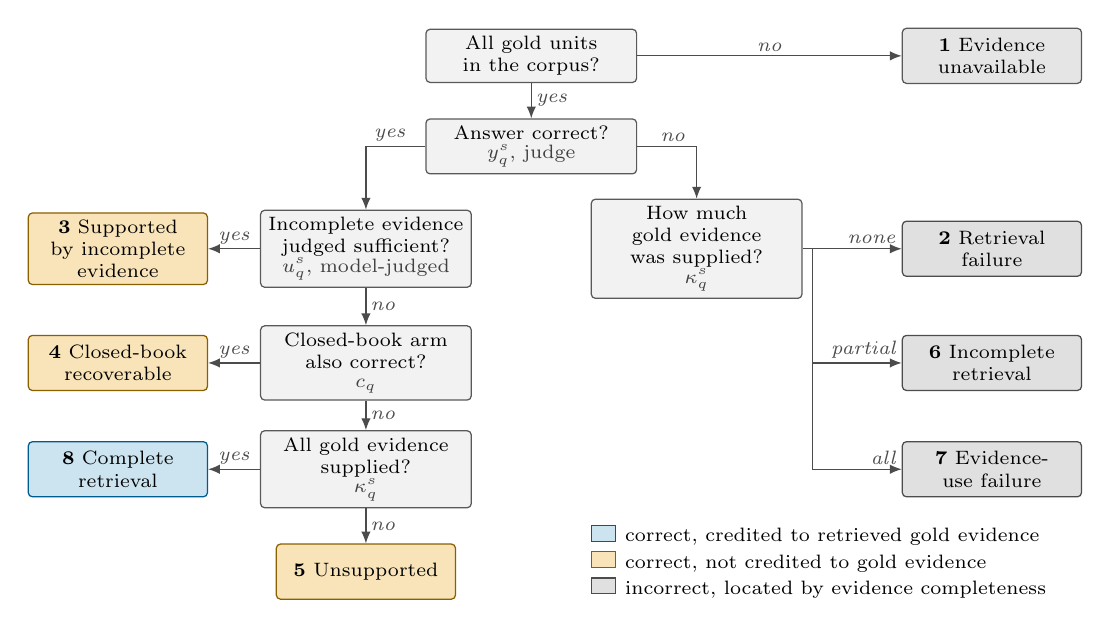
\begin{tikzpicture}[
  q/.style  = {box, fill=black!5, text width=25mm},
  st/.style = {box, text width=21mm, minimum height=7mm},
  ok/.style = {st, fill=cCredit!20, draw=cCredit!80!black},
  nc/.style = {st, fill=cNotCredit!28, draw=cNotCredit!60!black},
  er/.style = {st, fill=black!12, draw=black!70},
  na/.style = {st, fill=black!10},
]
\def\qx{2.1}   % question columns
\def\lx{5.25}   % leaf columns
\def\rx{5.85}   % right-hand leaf column
% Root and correctness split
\node[q] (avail) at (0,0)        {All gold units in the corpus?};
\node[na] (s1)   at (\rx,0)      {\textbf{1} Evidence unavailable};
\node[q] (corr)  at (0,-1.15)    {Answer correct?\\[-1pt]\textcolor{black!75}{$y_q^s$, judge}};

% Correct branch: questions in a column, leaves to the left
\node[q] (suff)  at (-\qx,-2.45) {Incomplete evidence judged sufficient?\\[-1pt]\textcolor{black!75}{$u_q^s$, model-judged}};
\node[q] (cb)    at (-\qx,-3.9) {Closed-book arm also correct?\\[-1pt]\textcolor{black!75}{$c_q$}};
\node[q] (cmp1)  at (-\qx,-5.25) {All gold evidence supplied?\\[-1pt]\textcolor{black!75}{$\kappa_q^s$}};
\node[nc] (s3)   at (-\lx,-2.45) {\textbf{3} Supported by incomplete evidence};
\node[nc] (s4)   at (-\lx,-3.9) {\textbf{4} Closed-book recoverable};
\node[ok] (s8)   at (-\lx,-5.25) {\textbf{8} Complete retrieval};
\node[nc] (s5)   at (-\qx,-6.55)  {\textbf{5} Unsupported};

% Incorrect branch: one question, three leaves to the right
\node[q] (gold)  at (\qx,-2.45) {How much gold evidence was supplied?\\[-1pt]\textcolor{black!75}{$\kappa_q^s$}};
\node[er] (s2)   at (\rx,-2.45) {\textbf{2} Retrieval failure};
\node[er] (s6)   at (\rx,-3.9) {\textbf{6} Incomplete retrieval};
\node[er] (s7)   at (\rx,-5.25) {\textbf{7} Evidence-use failure};

% Edges
\draw[arr] (avail) -- node[lab, above] {no} (s1);
\draw[arr] (avail) -- node[lab, right] {yes} (corr);
\draw[arr] (corr.west) -| node[lab, above, pos=0.3] {yes} (suff.north);
\draw[arr] (corr.east) -| node[lab, above, pos=0.3] {no} (gold.north);

\draw[arr] (suff) -- node[lab, above] {yes} (s3);
\draw[arr] (suff) -- node[lab, right] {no} (cb);
\draw[arr] (cb)   -- node[lab, above] {yes} (s4);
\draw[arr] (cb)   -- node[lab, right] {no} (cmp1);
\draw[arr] (cmp1) -- node[lab, above] {yes} (s8);
\draw[arr] (cmp1) -- node[lab, right] {no} (s5);

\coordinate (gsplit) at ($(gold.east)!0.1!(s2.west)$);
\draw[arr] (gold.east) -- (s2.west) node[lab, above left, pos=1, inner xsep=2pt] {none};
\draw[arr] (gsplit) |- (s6.west) node[lab, above left, pos=1, inner xsep=2pt] {partial};
\draw[arr] (gsplit) |- (s7.west) node[lab, above left, pos=1, inner xsep=2pt] {all};

% Legend, under the incorrect branch
\node[anchor=north west, inner sep=0pt] at (0.75,-5.95) {%
  \scriptsize
  \begin{tabular}{@{}l@{\hspace{1.2mm}}l@{}}
  \tikz\draw[fill=cCredit!20, draw=cCredit!80!black] (0,0) rectangle (3mm,2mm); & correct, credited to retrieved gold evidence \\[1pt]
  \tikz\draw[fill=cNotCredit!28, draw=cNotCredit!60!black] (0,0) rectangle (3mm,2mm); & correct, not credited to gold evidence \\[1pt]
  \tikz\draw[fill=black!12, draw=black!70] (0,0) rectangle (3mm,2mm); & incorrect, located by evidence completeness
  \end{tabular}};
\end{tikzpicture}
\caption{Decision flow that assigns each answer an evidence state, following
the rules of Table~\ref{tab:states}, with the three state groups in
separate colours.}
\label{fig:states}
\end{figure*}


\begin{table*}[!tbp]
\centering
\caption{Evidence-attribution states, applied in order. The first matching
rule assigns the state.}
\label{tab:states}
\footnotesize
\begin{tabular}{@{}c>{\raggedright\arraybackslash}p{0.22\textwidth}>{\raggedright\arraybackslash}p{0.40\textwidth}>{\raggedright\arraybackslash}p{0.24\textwidth}@{}}
\toprule
& State & Rule & Source of the decision \\
\midrule
1 & Evidence unavailable & a gold unit is absent from the searchable corpus & corpus contents \\
2 & Retrieval failure & $\kappa_q^{s}=\text{none}$ and $y_q^{s}=0$ & provenance \\
3 & Supported by incomplete evidence & $y_q^{s}=1$, $\kappa_q^{s}\neq\text{complete}$, and $u_q^{s}=1$ & model-judged sufficiency \\
4 & Closed-book recoverable & $y_q^{s}=1$ and $c_q=1$ & closed-book arm \\
5 & Unsupported & $y_q^{s}=1$ and $\kappa_q^{s}\neq\text{complete}$ & residual \\
6 & Incomplete retrieval & $y_q^{s}=0$ and $\kappa_q^{s}=\text{partial}$ & provenance \\
7 & Evidence-use failure & $y_q^{s}=0$ and $\kappa_q^{s}=\text{complete}$ & provenance, score \\
8 & Complete retrieval & $y_q^{s}=1$ and $\kappa_q^{s}=\text{complete}$ & provenance, score \\
\bottomrule
\end{tabular}
\end{table*}

Only state~8 is a correct answer that can be credited to the retrieved gold
evidence. States 3--5 are correct answers that cannot; states 2, 6, and 7 are
errors that locate the failure in retrieval, in partial retrieval, or in the
generator's use of complete evidence. State~3 depends on a model judgement and
is reported as model-judged (Section~\ref{sec:validation}).

\subsection{Access and use decomposition}

Let $p_s(k)=\Pr[\kappa_q^{s}=k]$ and $a_s(k)=\Pr[y_q^{s}=1\mid\kappa_q^{s}=k]$
for $k\in\{\text{complete},\text{partial},\text{none}\}$. For a treatment
system $t$ and a reference system $r$ evaluated on the same questions and
generator,
\begin{equation}
\label{eq:decomp}
\underbrace{\mathrm{Acc}_t-\mathrm{Acc}_r}_{\Delta}
= \underbrace{\sum_k \bigl(p_t(k)-p_r(k)\bigr)\,a_r(k)}_{\Delta_{\text{access}}}
\; + \;
\underbrace{\sum_k p_t(k)\bigl(a_t(k)-a_r(k)\bigr)}_{\Delta_{\text{use}}} .
\end{equation}
The identity follows from $p_t a_t - p_r a_r = (p_t-p_r)a_r + p_t(a_t-a_r)$
summed over strata. $\Delta_{\text{access}}$ is the accuracy change expected
if the treatment only moved questions between completeness strata and the
generator kept the reference system's per-stratum accuracy.
$\Delta_{\text{use}}$ is the change in per-stratum accuracy, weighted by the
treatment's stratum shares. A retrieval-stage intervention that works by
recovering missing evidence should show a positive access term; a
prompt-side intervention such as +KG cannot change $p(k)$ by construction, so
its whole effect falls in the use term. The decomposition is descriptive
rather than causal. The question mix inside each stratum can change between
systems, and we report $\Delta_{\text{use}}$ with that caveat.
Figure~\ref{fig:decomp} shows why the split matters. A modest net gain can
combine a larger access gain with a use loss, for example when extra passages
recover gold evidence but also distract the generator.

% Access/use decomposition (Eq.~\ref{eq:decomp}) with illustrative values.
% Reference r: p = (0.40, 0.40, 0.20), a = (0.20, 0.40, 0.90) -> Acc 0.42
% Treatment t: p = (0.20, 0.35, 0.45), a = (0.20, 0.40, 0.80) -> Acc 0.54
% Access = -0.04 - 0.02 + 0.225 = +0.165; use = 0.45 * (-0.10) = -0.045.
% Bar length 9 cm = all questions.
\begin{figure}[t]
\centering
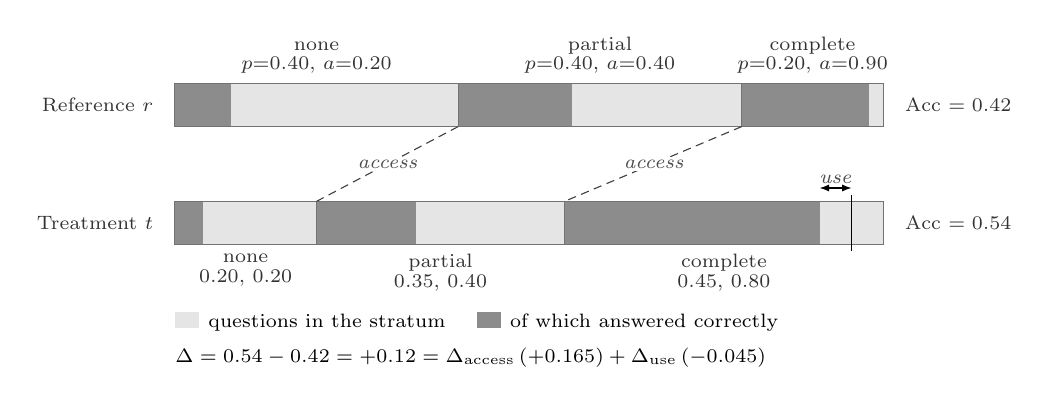
\begin{tikzpicture}[
  seg/.style  = {draw=black!55, line width=0.35pt},
  slab/.style = {font=\scriptsize, align=center, text=black!80},
]
\def\h{0.55}
% Reference bar (y = 1.5 .. 2.05)
\begin{scope}[shift={(0,1.5)}]
  \fill[black!10]        (0,0)   rectangle (3.6,\h);
  \fill[black!45]        (0,0)   rectangle (0.72,\h);
  \fill[black!10]  (3.6,0) rectangle (7.2,\h);
  \fill[black!45]  (3.6,0) rectangle (5.04,\h);
  \fill[black!10]     (7.2,0) rectangle (9.0,\h);
  \fill[black!45]     (7.2,0) rectangle (8.82,\h);
  \draw[seg] (0,0) rectangle (9,\h);
  \draw[seg] (3.6,0) -- (3.6,\h) (7.2,0) -- (7.2,\h);
  \node[slab, above] at (1.8,\h) {none\\[-1pt]$p{=}0.40$, $a{=}0.20$};
  \node[slab, above] at (5.4,\h) {partial\\[-1pt]$p{=}0.40$, $a{=}0.40$};
  \node[slab, above] at (8.1,\h) {complete\\[-1pt]$p{=}0.20$, $a{=}0.90$};
  \node[slab, anchor=east] at (-0.15,\h/2) {Reference $r$};
  \node[slab, anchor=west] at (9.15,\h/2) {Acc $=0.42$};
\end{scope}
% Treatment bar (y = 0 .. 0.55)
\fill[black!10]        (0,0)    rectangle (1.8,\h);
\fill[black!45]        (0,0)    rectangle (0.36,\h);
\fill[black!10]  (1.8,0)  rectangle (4.95,\h);
\fill[black!45]  (1.8,0)  rectangle (3.06,\h);
\fill[black!10]     (4.95,0) rectangle (9.0,\h);
\fill[black!45]     (4.95,0) rectangle (8.19,\h);
\draw[seg] (0,0) rectangle (9,\h);
\draw[seg] (1.8,0) -- (1.8,\h) (4.95,0) -- (4.95,\h);
\node[slab, below] at (0.9,0)   {none\\[-1pt]$0.20$, $0.20$};
\node[slab, below] at (3.375,0) {partial\\[-1pt]$0.35$, $0.40$};
\node[slab, below] at (6.975,0) {complete\\[-1pt]$0.45$, $0.80$};
\node[slab, anchor=east] at (-0.15,\h/2) {Treatment $t$};
\node[slab, anchor=west] at (9.15,\h/2) {Acc $=0.54$};

% Access: stratum boundaries move between the bars
\draw[densely dashed, black!75] (3.6,1.5) -- (1.8,\h);
\draw[densely dashed, black!75] (7.2,1.5) -- (4.95,\h);
\node[lab, fill=white, inner sep=1pt] at (6.08,1.02) {access};
\node[lab, fill=white, inner sep=1pt] at (2.7,1.02) {access};

% Use: in the complete stratum the treatment's accuracy (0.80) falls short of
% the reference's (0.90); the gap is 0.45 x 0.10 = 0.045 of all questions.
\draw[black, line width=0.6pt] (8.595,-0.08) -- (8.595,\h+0.08);
\draw[{Latex[length=1.2mm]}-{Latex[length=1.2mm]}, black] (8.19,\h+0.17) -- (8.595,\h+0.17);
\node[lab, anchor=south] at (8.39,\h+0.17) {use};

% Legend
\node[anchor=north west, inner sep=0pt] at (0,-0.85) {%
  \scriptsize
  \begin{tabular}{@{}l@{\hspace{1.2mm}}l@{\hspace{4mm}}l@{\hspace{1.2mm}}l@{}}
  \tikz\fill[black!10] (0,0) rectangle (3mm,2mm); & questions in the stratum &
  \tikz\fill[black!45] (0,0) rectangle (3mm,2mm); & of which answered correctly \\
  \end{tabular}};
\node[anchor=north west, inner sep=0pt, font=\scriptsize] at (0,-1.3)
  {$\Delta = 0.54 - 0.42 = +0.12 = \Delta_{\text{access}}\,(+0.165) + \Delta_{\text{use}}\,(-0.045)$};
\end{tikzpicture}
\caption{Access and use terms of Eq.~\eqref{eq:decomp} for illustrative
values. Each bar is the full question set divided by evidence completeness,
with segment width $p$ and the dark part of each segment the share answered
correctly, $a$. Dashed lines show questions moving between strata, and the
black tick marks the treatment's lower accuracy in the complete stratum.}
\label{fig:decomp}
\end{figure}


\subsection{Research questions and pre-specified hypotheses}
\label{sec:rqs}

The research questions, hypotheses, and primary outcomes below were fixed
before any results were collected.

The first research question (RQ1) asks whether graph augmentation improves
retrieval and answer quality after controlling for candidate-set size and
non-graph query expansion. We predicted (H1) that on HotpotQA bridge questions
+KGret achieves higher gold-evidence completeness and higher exact match than
dense top-5 retrieval at the same budget of five passages. The primary outcome
is the paired difference in exact match, +KGret minus dense top-5, pooled over
generators with a question-level cluster bootstrap.

The second (RQ2) asks whether graph augmentation is beneficial primarily under
measurable evidence deficits. We predicted (H2) that the +KGret minus dense
top-5 difference is larger on bridge questions, where baseline completeness is
low, than on comparison questions, where it is high, and that on bridge
questions most of it lies in $\Delta_{\text{access}}$.

The third (RQ3) asks how caption, corpus-text, and model-prior paths change
the estimated value of multimodal retrieval. We predicted (H3) that on SPIQA
human-authored figure questions the estimated gain of CLIP-retrieved pixels
over text-only retrieval is larger on caption-flagged items than on
caption-screened items, and that on screened items it shrinks further when
corpus-text-recoverable and closed-book-recoverable items are removed.

The fourth (RQ4) asks how much end-to-end failure is attributable to
retrieval, evidence completeness, evidence use, or unsupported generation. It
is descriptive and is reported as state distributions per set, system, and
generator tier.


% =========================================================================
\section{Experimental Setup}
\label{sec:setup}
% =========================================================================

\subsection{Corpora and question sets}
\label{sec:corpora}

Table~\ref{tab:qsets} lists every question set, who wrote it, and how it is
used. Headline claims rest only on the two sets written by benchmark
annotators. Model-authored sets are used as mechanism tests and are reported
in separate tables.

\begin{table*}[!tbp]
\centering
\caption{Question sets. ``Role'' states whether a set carries headline claims
or serves as a mechanism test. Graph-seeded items were generated from entities
in the same graph that +KGret searches and are never pooled with other sets.}
\label{tab:qsets}
\footnotesize
\resizebox{\textwidth}{!}{%
\begin{tabular}{@{}llrlll@{}}
\toprule
Corpus & Set & $n$ & Authored by & Primary metric & Role \\
\midrule
HotpotQA  & bridge                 & 100 & benchmark annotators & EM, F1; containment, judge & headline (RQ1, RQ2) \\
HotpotQA  & comparison             & 100 & benchmark annotators & EM, F1; containment, judge & headline control (RQ2) \\
SPIQA     & native figure, screened & 150 & benchmark annotators & judge accuracy & headline (RQ3) \\
SPIQA     & native figure, caption-flagged & 132 & benchmark annotators & judge accuracy & leakage contrast (RQ3) \\
SPIQA     & cross-paper multi-hop  & 50  & DeepSeek, graph-seeded & judge accuracy & mechanism only \\
PubLayNet & pixel-only figure      & 35 & Claude Haiku~4.5 & judge accuracy & mechanism (RQ3) \\
\bottomrule
\end{tabular}}
\end{table*}

The HotpotQA corpus pools the context paragraphs of the sampled questions,
drawn from the benchmark's distractor setting~\cite{yang2018hotpotqa}, 5{,}910 Wikipedia
articles split into 10{,}108 chunks, from which 72{,}946 triples were
extracted, forming a graph of 76{,}846 nodes and 71{,}540 distinct edges. One
provenance unit is one Wikipedia article and each question has two gold
articles. Bridge questions name one entity and require a second article
reached through it; comparison questions name both entities. The split
between bridge and comparison questions is therefore a within-corpus control
for evidence deficit. Questions, answers, and supporting
facts are the benchmark's own.

The SPIQA corpus contains 100 papers from the curated test-A split of
SPIQA~\cite{spiqa}, with 8{,}474 text chunks from the distributed TeX
paragraphs, 978 figure and table crops, and 50{,}123 extracted triples. SPIQA's
annotators wrote 579 question--answer pairs over these papers, each tied to
one crop. A caption-leakage screen (Section~\ref{sec:leakscreen}) flags 132
items whose reference answer appears in the pipeline or author caption. From
the remaining 447 we sampled 150 with a fixed seed as the primary set. The 132
flagged items form a contrast set for RQ3 (Figure~\ref{fig:funnel}). 40 of the
579 questions name their own modality (for example ``in the table''); we
report this rather than editing a published benchmark. SPIQA is public, so
prior exposure is measured with the closed-book arm rather than assumed away.

% SPIQA native question filtering. Counts 579 / 132 / 447 / 150 are from
% data/questions/questions_spiqa_native*.json (leakage_status field); the
% sample seed is configs/*.json "seed". Later counts come from the runs.
\begin{figure}[t]
\centering
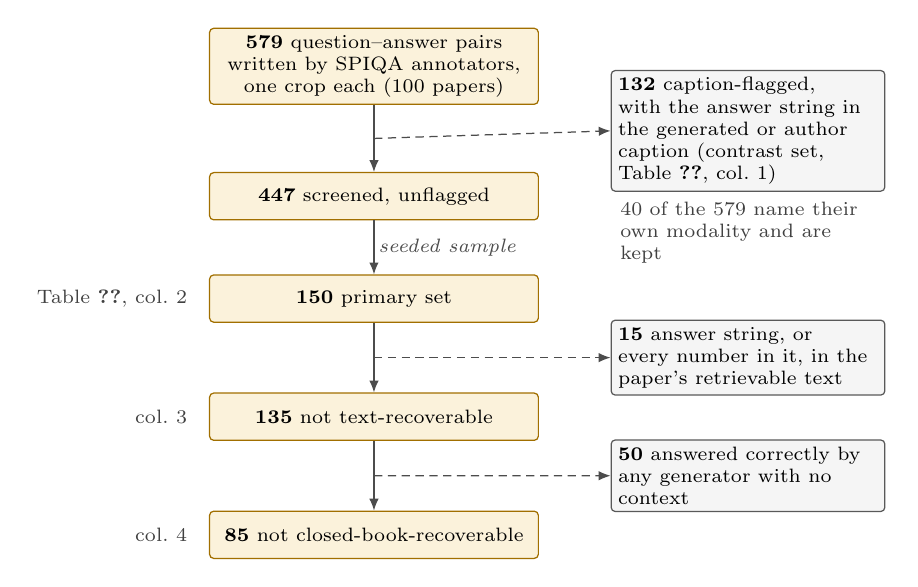
\begin{tikzpicture}[
  main/.style = {box, fill=cVis!14, draw=cVis!70!black, text width=40mm},
  side/.style = {box, fill=black!4, text width=33mm, align=left},
  tag/.style  = {font=\scriptsize, text=black!75, anchor=east, align=right},
]
\node[main] (m1) at (0,0) {\textbf{579} question--answer pairs written by SPIQA annotators, one crop each (100 papers)};
\node[main] (m2) at (0,-1.65) {\textbf{447} screened, unflagged};
\node[main] (m3) at (0,-2.95) {\textbf{150} primary set};
\node[main] (m4) at (0,-4.45) {\textbf{135} not text-recoverable};
\node[main] (m5) at (0,-5.95) {\textbf{85} not closed-book-recoverable};

\draw[arr] (m1) -- (m2) coordinate[midway] (c1);
\draw[arr] (m2) -- node[lab, right] {seeded sample} (m3);
\draw[arr] (m3) -- (m4) coordinate[midway] (c3);
\draw[arr] (m4) -- (m5) coordinate[midway] (c4);

\node[side] (x1) at (4.75,-0.82) {\textbf{132} caption-flagged, with the answer string in the generated or author caption (contrast set, Table~\ref{tab:mm}, col.~1)};
\node[side] (x3) at (4.75,-3.7)  {\textbf{15} answer string, or every number in it, in the paper's retrievable text};
\node[side] (x4) at (4.75,-5.2)  {\textbf{50} answered correctly by any generator with no context};
\draw[arr, densely dashed] (c1) -- (x1.west);
\draw[arr, densely dashed] (c3) -- (x3.west);
\draw[arr, densely dashed] (c4) -- (x4.west);

% Which column of the multimodal table each set feeds
\node[tag] at (-2.25,-2.95) {Table~\ref{tab:mm}, col.~2};
\node[tag] at (-2.25,-4.45) {col.~3};
\node[tag] at (-2.25,-5.95) {col.~4};
\node[font=\scriptsize, text=black!75, anchor=north west, text width=33mm, align=left]
  at (x1.south west) {40 of the 579 name their own modality and are kept};
\end{tikzpicture}
\caption{Filtering of SPIQA's human-written figure questions. Each dashed exit
removes one textual route to the answer, and the column labels give the
column of Table~\ref{tab:mm} that each set feeds.}
\label{fig:funnel}
\end{figure}


The PubLayNet corpus contains 1{,}000 pages from the small-publaynet-wds
release of PubLayNet
\cite{lhoestq_small_publaynet_wds,zhong2019publaynet}. Text regions are
processed with Tesseract OCR; figure and table regions are kept as crops,
captioned once with GPT-4o. For this study the corpus was rebuilt from the
same pages with Tesseract~5.5.3, so its OCR text, captions, and extracted graph
differ from those of~\cite{jonah2026whendo}. The figure crops, which the
questions refer to, are cut from the dataset's own region boxes and are
unchanged. Because figure content never enters the OCR text,
PubLayNet is an obscure-corpus reference point on which text recovery of
figure answers is closed by construction.

The remaining sets were written by models. Claude Haiku~4.5 wrote the
PubLayNet figure questions and DeepSeek-Chat the text questions, at
temperature~0. Every
model-authored item is reviewed by a model from a different family under the
rules in Section~\ref{sec:validation}, and rejection rates are reported.

\subsection{Shared processing}

Across corpora, text is split into 500-character windows with 50-character
overlap and embedded with OpenAI's text-embedding-3-small model
\cite{openai2024embeddings}; crops are embedded with CLIP ViT-B/32
\cite{radford2021clip}; both are indexed with FAISS under cosine similarity
\cite{johnson2019faiss}. GPT-4o-mini extracts subject--relation--object
triples once per chunk; triples keep the identifier of their source chunk and
are stored in a directed NetworkX graph~\cite{hagberg2008networkx}.

\subsection{Systems and evidence controls}
\label{sec:systems}

Let $R_k(q)$ be the dense top-$k$ passages. The generation-stage graph system,
+KG, supplies $R_3(q)$ plus at most eight triples whose matched entity occurs in
$q$ (whole-word, at least five characters) and whose source chunk is already
in $R_3(q)$:
\begin{equation}
R_{\text{kg}}(q)=\bigl\{e\in\mathcal{E}:\eta(e)\sqsubseteq q,\ \pi(e)\in\pi(R_3(q))\bigr\}.
\end{equation}
+KG can only restructure evidence already retrieved. +KGret injects no triples;
it adds up to $B=2$ chunks from provenance units linked to the matched
entities and not already retrieved, ranked by query similarity:
\begin{equation}
\label{eq:kgret}
R_{\text{kgret}}(q)=R_3(q)\cup\operatorname{Top}_{B}\bigl\{c:\pi(c)\in\mathrm{pages}_h(\mathcal{E}(q))\setminus\pi(R_3(q))\bigr\}.
\end{equation}
Here $\mathcal{E}(q)$ is the set of graph nodes whose name occurs as a whole
word in $q$ (at least five characters), and $\mathrm{pages}_h$ collects the
provenance units of every triple incident to those nodes ($h=1$) and, for
$h=2$, also of triples incident to their neighbours, capped at 20 neighbours
per node. HotpotQA uses $h=2$, because a bridge question never names the
bridge entity; SPIQA and PubLayNet use $h=1$.
Figure~\ref{fig:bridge} traces one bridge question through these rules.
+KGret therefore receives at most five passages (Figure~\ref{fig:design}).

% Worked +KGret example on an evaluated bridge question
% (5ababbe9554299232ef4a38a). Every triple shown is in
% data/graphs/triples_cache_hotpotqa_corpus.json (node names lower-cased by
% normalise_entity); matching and h = 2 expansion follow bridge_pages() in
% src/multimodal_graph_rag/retrieval/graph_expansion.py. Pool size, the two
% chunks kept, and dense top-3 are from
% artifacts/runs/retrieval_ab_questions_hotpotqa_bridge_h2.json.
\begin{figure*}[t]
\centering
\newcommand{\relname}[1]{{\scriptsize\upshape\textcolor{black!75}{#1}}}
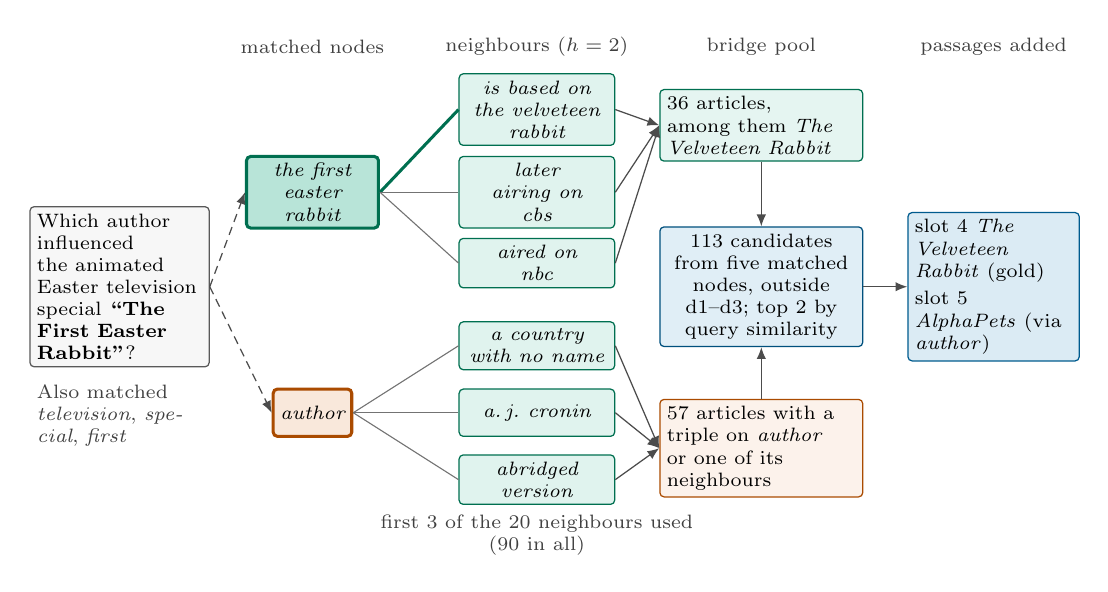
\begin{tikzpicture}[
  ent/.style   = {box, fill=cGraph!12, draw=cGraph!70!black, font=\scriptsize\itshape},
  hit/.style   = {ent, line width=1.1pt, fill=cGraph!28, text width=15mm},
  clash/.style = {ent, line width=1.1pt, fill=cErr!14, draw=cErr!80!black},
  nb/.style    = {ent, text width=18mm},
  pool/.style  = {box, text width=24mm, align=left},
  head/.style  = {font=\scriptsize, text=black!75},
]
% Question
\node[box, fill=black!3, text width=21mm, align=left] (q) at (0,0)
  {Which author influenced the animated Easter television special
  \textbf{``The First Easter Rabbit''}?};
\node[font=\scriptsize, text=black!75, below=1mm of q, text width=21mm, align=left]
  {Also matched \emph{television}, \emph{special}, \emph{first}};

% Matched nodes
\node[hit]   (fer) at (2.45,1.2)  {the first easter rabbit};
\node[clash] (au)  at (2.45,-1.6) {author};
\draw[arr, densely dashed] (q.east) -- (fer.west);
\draw[arr, densely dashed] (q.east) -- (au.west);

% Neighbours; the relation of each triple is printed above the neighbour
\node[nb] (vr)  at (5.3,2.25) {\relname{is based on}\\ the velveteen rabbit};
\node[nb] (rb)  at (5.3,1.2)  {\relname{later airing on}\\ cbs};
\node[nb] (nbc) at (5.3,0.3)  {\relname{aired on}\\ nbc};
\draw[line width=1.1pt, cGraph!70!black] (fer.east) -- (vr.west);
\draw[black!55] (fer.east) -- (rb.west);
\draw[black!55] (fer.east) -- (nbc.west);

\node[nb] (cw)  at (5.3,-0.75) {a country with no name};
\node[nb] (ajc) at (5.3,-1.6)  {a.\,j.\ cronin};
\node[nb] (abr) at (5.3,-2.45) {abridged version};
\draw[black!55] (au.east) -- (cw.west);
\draw[black!55] (au.east) -- (ajc.west);
\draw[black!55] (au.east) -- (abr.west);
\node[font=\scriptsize, text=black!75, align=center] at (5.3,-3.15)
  {first 3 of the 20 neighbours used\\ (90 in all)};

% Bridge pools and selection
\node[pool, fill=cGraph!10, draw=cGraph!70!black] (p1) at (8.15,2.05)
  {36 articles, among them \emph{The Velveteen Rabbit}};
\node[pool, fill=cErr!8, draw=cErr!80!black] (p2) at (8.15,-2.05)
  {57 articles with a triple on \emph{author} or one of its neighbours};
\node[box, fill=cText!12, draw=cText!70!black, text width=24mm] (sel) at (8.15,0.0)
  {113 candidates from five matched nodes, outside d1--d3; top 2 by query similarity};
\foreach \n in {vr,rb,nbc} \draw[arr] (\n.east) -- (p1.west);
\foreach \n in {cw,ajc,abr} \draw[arr] (\n.east) -- (p2.west);
\draw[arr] (p1) -- (sel);
\draw[arr] (p2) -- (sel);

% Outcome
\node[box, fill=cCredit!14, draw=cCredit!80!black, text width=20mm, align=left]
  (out) at (11.1,0.0)
  {slot 4 \emph{The Velveteen Rabbit} (gold)\\[2pt] slot 5 \emph{AlphaPets}
  (via \emph{author})};
\draw[arr] (sel) -- (out);

% Column headings
\node[head] at (2.45,3.05) {matched nodes};
\node[head] at (5.3,3.05)  {neighbours ($h=2$)};
\node[head] at (8.15,3.05) {bridge pool};
\node[head] at (11.1,3.05) {passages added};
\end{tikzpicture}
\caption{One evaluated HotpotQA bridge question traced through +KGret, using
triples from the extracted graph. The bold edge is the triple that reaches the
gold article, and the vermilion node and pool mark a generic match whose
articles compete for the same two slots. The other three matched nodes add
candidates of their own, so the two pools shown sum to less than 113.}
\label{fig:bridge}
\end{figure*}


The most direct comparator is dense top-5, $R_5(q)$, which asks whether the
graph or simply the two extra slots carries any gain. Two comparators replace
the dense ranking altogether, BM25 top-5~\cite{robertson2009bm25} over the
same chunks and a hybrid that fuses the top 100 of the dense and BM25 rankings
by reciprocal rank with the usual constant of 60~\cite{cormack2009rrf}. Two
others keep $R_3(q)$ and fill the remaining slots without following any graph
edge, adding at most one chunk per unit and never a unit already in $R_3(q)$.
Lexical entity expansion starts from the same entities $\mathcal{E}(q)$ as
+KGret but finds their names in chunk text, adding up to two of the
best-ranked chunks that contain one. Like +KGret it can add fewer than two.
Random padding adds two random chunks as a floor for any expansion. The
published graph comparator supplies the top five passages from
HippoRAG\,2~\cite{gutierrez2025hipporag2}, indexed over the same chunks with
GPT-4o-mini for open information extraction and text-embedding-3-small for
embeddings, and its rankings were fixed before any answer was generated. All of these arms, +KGret included,
share one prompt and present their passages without any mark of the arm that
selected them, so they differ in retrieval alone.

For figures, CLIP ranks crops by text--image similarity, and the generator
receives $R_5(q)$ together with either the top-ranked crop as pixels or the
captions of the top three crops. Pixels are supplied only for figure questions.

Five further arms replace part or all of the context instead of adding to
it. The closed-book arm supplies nothing, the shuffled arm supplies unrelated
passages of matched length, the oracle arm supplies passages from every gold
unit, and the partial-gold arm supplies passages from the first gold unit
only. For figure questions the oracle-image arm supplies $R_5(q)$ with the
gold crop in place of the retrieved one, or its caption in the caption
condition. Its difference from the pixel arm is therefore image retrieval
alone, and the errors it still makes are failures to read the figure.

\subsection{Generators}
\label{sec:generators}

Generators are grouped by capability tier, because a stronger generator can
both raise closed-book accuracy and use evidence better, and either could change
the size of an augmentation effect. Tier is therefore analysed as a moderator,
and the generators are never treated as independent replications
(Section~\ref{sec:stats}).

\begin{table}[t]
\caption{Generator models, all accessed through OpenRouter, with prices in USD
per million input and output tokens on 20 October 2026.}
\label{tab:models}
\centering
\footnotesize
\begin{tabular}{@{}lllr@{\,/\,}l@{}}
\toprule
Tier & Model & Weights & \multicolumn{2}{c}{\$/1M} \\
\midrule
Earlier, small & Llama~4 Scout         & open        & 0.10 & 0.30 \\
Current, small & GPT-6 Luna            & proprietary & 0.10 & 0.50 \\
               & Gemma~4 31B          & open        & 0.14 & 0.40 \\
Current, strong & Gemini~3.8 Flash     & proprietary & 0.825 & 4.125 \\
                & Qwen~3.8 Max         & proprietary & 2.00 & 6.00 \\
\bottomrule
\end{tabular}
\end{table}

Llama~4 Scout is kept from the four generators of~\cite{jonah2026whendo} for
continuity, and the rest of the roster is refreshed. GPT-4o-mini is replaced
by GPT-6 Luna, which OpenAI names as its successor and which remains
available after GPT-4o-mini is withdrawn on 14 January 2027. Llama~4 Maverick
is replaced by Gemma~4 31B as a current open-weight model. Llama~4 Scout is
served by DeepInfra, the provider used in that study, and Gemma~4 31B by
Crusoe or Novita, which both serve its unquantised weights. Within each arm every model receives the
same prompt and evidence. The passage arms instruct the generator to answer
only from the supplied context and to say it does not know otherwise, while
the closed-book arm asks it to answer from its own knowledge. The model
version and serving provider are recorded for each answer.

The strong tier is Gemini~3.8 Flash and Qwen~3.8 Max, the latter as its
dated snapshot of 2 September 2026. Neither family supplies a judge. Both
models, like GPT-6 Luna, reason before answering,
and their reasoning is left at the provider default for every arm.

\subsection{Metrics}
\label{sec:metrics}

Retrieval is scored against gold provenance. For gold units $G_q$ and ranked
units $(r_1,\dots,r_k)$, Recall@$k$ is the fraction of questions with $G_q\cap\{r_1..r_k\}\neq
\varnothing$, MRR uses the rank of the first gold unit, and completeness is the
fraction with $G_q\subseteq\{r_1..r_k\}$. For figure questions only the
top-ranked crop reaches the generator, so Recall@1 is the operational ceiling;
Recall@3 and @5 are reported as diagnostics only.

Answers are scored differently on the two headline corpora. On HotpotQA the
primary outcome is exact match, with token F1 and answer containment reported
beside it; these use the benchmark's normalisation and the annotators'
reference answers, so no judge model is involved. SPIQA-native answers are discursive and exact match is too strict
for them, so the primary outcome is the binary accuracy verdict of the primary
judge, reported with F1.

Exact match turned out to measure answer format more than answer content on
HotpotQA. Gemma 4 31B and Gemini 3.8 Flash answer in a full sentence rather
than with the answer span, so with both gold articles supplied their exact
match on bridge questions is 0.01 and 0.04, against judge accuracy of 0.91
and 0.95. Comparison references are mostly \emph{yes}, \emph{no}, or a name,
and on that set exact match is at most 0.06 for every generator and system. We
report exact match and its paired tests as pre-specified. Because it cannot
separate systems for most generators, we also report the same paired analysis
for answer containment, which checks whether the normalised reference occurs in
the normalised answer and involves no judge, and for the accuracy verdict of
DeepSeek V4 Pro. Both were pre-specified as secondary measures; giving them
equal weight in the text was decided after the results were seen, and
conclusions that rest on them are marked as such.

Faithfulness to the supplied context is judged on the text sets and not on
the figure sets, and no faithfulness result enters a comparison reported here.
Relevance is not scored; in the earlier study it was nearly always positive and
carried no information.

% =========================================================================
\section{Validation of Model-Based Instruments}
\label{sec:validation}
% =========================================================================

The question authors, the graph extractor, the reviewers, and the judges in
this study are all language models. This section states how each
is checked and what therefore cannot be claimed.

\subsection{Judges}
\label{sec:judges}

\begin{table}[t]
\caption{Judges and their roles.}
\label{tab:judges}
\centering
\footnotesize
\begin{tabular}{@{}>{\raggedright\arraybackslash}p{0.24\linewidth}l>{\raggedright\arraybackslash}p{0.38\linewidth}@{}}
\toprule
Role & Model & Coverage \\
\midrule
Primary, figure sets & GPT-6.1 Sol & accuracy on every output \\
Primary, text sets & DeepSeek V4 Pro & accuracy and faithfulness on every output \\
Second, figure sets  & DeepSeek V4 Pro & accuracy on a stratified 20\% of outputs \\
Second, HotpotQA     & GPT-6.1 Sol & accuracy on a stratified 20\% of outputs \\
Adjudicator          & Claude Opus~5.5 & outputs on which the two judges disagree \\
Sufficiency          & GPT-6.1 Sol & correct HotpotQA answers given incomplete gold evidence \\
Stability            & DeepSeek V4 Pro & stratified 20\% of text-set outputs, judged three more times \\
\bottomrule
\end{tabular}
\end{table}

Each judge writes a one-sentence justification and then gives its binary
verdict alone on the final line. A reply without such a line is requested
again, up to three times in all, with reasoning switched off once a reply has
used the whole output allowance, and no verdict is ever inferred from a reply
that lacks the line. Calls request temperature 0, which GPT-6.1 Sol and Claude
Opus~5.5 do not expose because they reason before answering, and the
justification and full reply are stored with every verdict.

Each judge is checked in three ways. For synthetic calibration, the judge
receives the reference answer as if it had been generated, which must score 1,
and the reference of a different question from the same set, which must score
0; the two error rates give false-negative and false-positive floors. This is a
sanity bound and not calibration against human labels. Agreement is measured
between the two judges, raw and as Cohen's $\kappa$, on the 20\% double-judged
sample. Stability is measured by
re-judging a stratified 20\% subset three times and reporting the flip rate.

On HotpotQA the text judge can also be checked against containment, which
uses the annotators' references and no model. Over the 12{,}969 non-empty
answers, the accuracy verdict of DeepSeek V4 Pro agrees with containment on
87.4\% of bridge answers (Cohen's $\kappa=0.75$) and 78.9\% of comparison
answers ($\kappa=0.56$), against 52\% and 35\% for exact match ($\kappa=0.16$
and 0.01). The disagreements run in both directions. Containment credits
answers that name the reference entity while declining to answer, which the
judge rejects, and the judge credits paraphrases that containment misses,
such as \emph{Ibn Arabi} for the reference \emph{ibn\,`Arab\={\i}}. Of the replies that open by
declining to answer, the judge accepted 0.8\% on bridge questions and 2.5\% on
comparison questions, 30 of them where the reference answer is \emph{no}.
Scoring all 60 of those replies as incorrect changes no paired difference in
judge accuracy reported here by more than 0.006 and leaves every conclusion
unchanged.
In the synthetic calibration on the 200 HotpotQA questions the judge accepted
all 200 reference answers and rejected all 200 decoys, so both error floors
are 0 with a 95\% upper bound of 1.5\%. Re-judged three more times, the
stratified 20\% of non-empty answers kept their verdict in 99.4\% of
re-judgements on bridge questions and 98.9\% on comparison questions, and
1.0\% and 1.7\% of those answers changed verdict at least once.

A second judge graded a stratified 20\% of the answers on each set, from the
question, the reference, and the answer, as the primary judge does. On HotpotQA
GPT-6.1 Sol agrees with DeepSeek V4 Pro on 98.9\% of 1{,}300 bridge answers
($\kappa=0.98$) and 98.6\% of 1{,}300 comparison answers ($\kappa=0.97$). On the
figure sets DeepSeek V4 Pro agrees with GPT-6.1 Sol on 96.0\% of 1{,}248 answers
($\kappa=0.91$), with 95.0\% on the screened set, 97.8\% on the flagged set,
92.9\% on the caption arms, and all 112 on PubLayNet. Claude Opus~5.5 graded the
82 disagreements and sided with the primary judge on 11 of the 32 on HotpotQA
and 40 of the 50 on the figure sets. Using its verdicts in place of the primary
judge's moves no paired judge difference on HotpotQA by more than 0.004 and none
of the multimodal tests of Section~\ref{sec:res-mm} by more than 0.007. Reported
results use the primary judge. Neither judge is checked against human labels, so
this agreement shows consistency and not correctness.

One judge shares a family with one generator. GPT-6.1 Sol and GPT-6 Luna are
both OpenAI models, so on the figure sets the primary judge grades one
generator from its own family. We keep a single judge across generators so that
generator rows remain comparable, and report the overlap as a limitation.
Over the 312 sampled GPT-6 Luna answers on those sets the second judge agrees
with GPT-6.1 Sol on 94.9\%, and each judge accepts 124 of them, so the sample
shows no leniency toward that generator. On the SPIQA cross-paper set, the judge (DeepSeek V4 Pro) and
the question author (DeepSeek-Chat) share a family; that set is a mechanism
test and carries no headline claim.

\subsection{Graph quality}

We check every triple in each graph against the chunk it was extracted from,
recording whether the subject, the object, or both occur in that chunk,
whether the relation string occurs, and how many surface forms merge into one
node. This establishes lexical grounding over the whole graph, not relation
correctness, which is estimated by model-judged precision on a stratified
sample of 300 triples. Table~\ref{tab:grounding} reports the check. Both
endpoints occur in the source chunk for 79\% of the HotpotQA triples, 64\% of
the SPIQA triples, and 30\% of the PubLayNet triples. The PubLayNet text comes
from OCR of page images, which may account for part of that gap. Only the
HotpotQA graph enters the headline comparisons. \tbd{Judged precision per
corpus.}

\begin{table}[t]
\caption{Lexical grounding of the extracted triples in their source chunks.
Rates are shares of all triples.}
\label{tab:grounding}
\centering
\footnotesize
\begin{tabular}{@{}lrrr@{}}
\toprule
 & HotpotQA & SPIQA & PubLayNet \\
\midrule
Chunks                         & 10{,}108 & 8{,}474 & 7{,}305 \\
Chunks with no triple          & 453      & 774     & 1{,}771 \\
Triples                        & 72{,}946 & 50{,}123 & 36{,}670 \\
Subject in chunk               & 0.95 & 0.89 & 0.67 \\
Object in chunk                & 0.83 & 0.70 & 0.42 \\
Both endpoints in chunk        & 0.79 & 0.64 & 0.30 \\
Relation string in chunk       & 0.57 & 0.52 & 0.41 \\
Surface forms merged into one node & 610 & 604 & 1{,}026 \\
\bottomrule
\end{tabular}
\end{table}

\subsection{Model review of model-authored questions}

Every model-authored item is reviewed by a model from a family that did not
author it, for answerability from its gold source, uniqueness of the
reference answer, and absence of modality cues; rejected items are removed and
the rejection rate is reported per set. \tbd{rejection rates.}

\subsection{Leakage screen}
\label{sec:leakscreen}

For every figure question the normalised reference answer (lower-cased,
punctuation and articles removed) is checked for containment in the crop's
generated caption, in the author caption where one exists, and in the source
document's retrievable text, and an answer that contains numbers is also
flagged when every one of them occurs there. Items that pass are labelled
\emph{screened-unflagged}, never \emph{verified}, because exact-string
screening misses paraphrased leakage. The closed-book arm bounds that leakage
from the other side.

\subsection{Author supervision}

\tbd{Pending agreement among the authors.} Two authors spot-check stratified
samples of judge verdicts (\tbd{50} per set), graph triples (\tbd{50} per
corpus), every leakage-flagged item, and \tbd{N} model-reviewed questions, and
report the share they would overturn. This is author supervision of the
instruments, not independent annotation, and is not used to compute
inter-annotator agreement.

% =========================================================================
\section{Statistical Analysis}
\label{sec:stats}
% =========================================================================

All comparisons are paired, so two systems are always compared on the same
questions with the same generator. For each primary difference we report the absolute
difference with a percentile bootstrap 95\% interval from 10{,}000
resamples of questions~\cite{efron1993bootstrap}, together with the counts of
discordant pairs. For retrieval completeness, which does not depend on the
generator, and within one generator, the test is an exact McNemar test on
those pairs~\cite{mcnemar1947}. Differences pooled over generators use a
question-level cluster bootstrap, which resamples questions and keeps all
generator outcomes for a resampled question together. Their test is a
sign-flip permutation test on the per-question mean difference across
generators, with 10{,}000 random sign assignments, so the five answers to one
question are never treated as independent. $p$-values are corrected with Holm's procedure~\cite{holm1979} within two
pre-specified families, one for the graph questions (RQ1, RQ2) and one for the
multimodal question (RQ3). In the graph family each answer measure is corrected
separately over the sixteen comparisons of an equal-budget or smaller arm with
dense top-5 on the two HotpotQA sets. In the multimodal family judge accuracy is
corrected over eight tests, namely pixels against text-only on each of the four
SPIQA columns of Table~\ref{tab:mm} and on PubLayNet, captions against text-only
on the screened set, and the two contrasts of H3. The first contrast compares
the gain on the flagged and screened sets, resampling each separately for its
interval and permuting set membership for its test. The second compares the gain
on the filtered screened items with the gain on all screened items, and its test
compares the kept items with the removed ones. The access and use terms of Eq.~\eqref{eq:decomp}
receive bootstrap intervals from the same resamples. Because that split
weights the access term by the reference system's per-stratum accuracy, its
terms depend on which system is the reference; we therefore also report the
symmetric split that averages the two orderings~\cite{kitagawa1955components}.

Table~\ref{tab:deviations} lists every change to the pre-specified plan made
after data collection began, with its reason. Results under the original
specification are reported wherever it can still be computed.

\begin{table*}[!tbp]
\centering
\caption{Changes to the pre-specified analysis plan made after data collection
began.}
\label{tab:deviations}
\scriptsize
\begin{tabular}{@{}>{\raggedright\arraybackslash}p{0.27\textwidth}>{\raggedright\arraybackslash}p{0.33\textwidth}>{\raggedright\arraybackslash}p{0.33\textwidth}@{}}
\toprule
Pre-specified & Change & Reason \\
\midrule
Seven generators (GPT-4o-mini, Gemini 3.1 Flash-Lite, Llama 4 Maverick and Scout, Qwen 3.7 Flash, Gemini 3.8 Flash, Qwen 3.8 Max) & Five generators; GPT-6 Luna replaces GPT-4o-mini, Gemma 4 31B replaces Llama 4 Maverick, and Gemini 3.1 Flash-Lite and Qwen 3.7 Flash are dropped & GPT-4o-mini is being withdrawn; two models were dropped for resource limits, keeping each tier; Mistral Small 4, first chosen for Maverick's place, could not be served at the request volume. No result from a removed generator is reported \\
Sufficiency of the non-gold context ($u$) & Sufficiency of the whole supplied context, judged only when the gold evidence is incomplete & The non-gold passages cannot be separated from a partial gold article in the supplied context \\
Access and use split for +KGret and +KG & Also for HippoRAG\,2, reported as exploratory & HippoRAG\,2 was the only arm that changed accuracy \\
Generator tier tested as a moderator & Effects described by tier, not tested & With one to two generators per tier a test of the interaction has no useful power \\
Generator replies capped at 800 tokens & Cap of 8{,}192; answers that reached 800 tokens generated again from the same evidence; 41 Qwen 3.8 Max answers that then reached 8{,}192 stay empty and count as incorrect & Hidden reasoning counts against the cap and left some answers empty \\
Exact match as the HotpotQA outcome, containment and judge secondary & All three reported with equal weight & Two generators answer in full sentences, and comparison references are single words, so exact match measures format \\
Answer containment as a substring test & Containment on token boundaries & The substring test matched ``no'' inside ``know'' and ``not'' \\
Exact McNemar test on pooled pairs & Sign-flip permutation test on per-question differences & Pooled pairs share questions across generators and are not independent \\
Correctness in the evidence states by exact match on HotpotQA & Judge accuracy on every set & As for the HotpotQA outcome \\
All 50 SPIQA cross-paper questions & 49 questions & One released question has no reference answer \\
Five generators on the figure sets & Four; Qwen 3.8 Max is not run on them & Resource limits; every tier keeps at least one generator \\
+both and shuffled arms on the figure sets, and caption arms on the flagged set & Not run & Resource limits; the arms H3 needs and the oracle-image arm were kept \\
Faithfulness and a second vision judge on 20\% of image-arm outputs & Faithfulness not judged on the figure sets; the second judge grades accuracy & Resource limits; accuracy is the primary outcome on these sets \\
Sufficiency judged on the figure sets & Not judged, so correct answers without the gold crop are counted together & Resource limits \\
PubLayNet caption-answerable, text, and multi-hop sets & Only the pixel-only figure set is run & Resource limits; these were mechanism and continuity sets \\
Primary arms repeated twice more on a stratified subset & Not run & Resource limits; hosted-model variability is not estimated \\
A Holm family for RQ3 without its tests listed & Eight tests, listed in Section~\ref{sec:stats} & The list was fixed after the arm means were seen and before any test was run \\\bottomrule
\end{tabular}
\end{table*}

% =========================================================================
\section{Results}
\label{sec:results}
% =========================================================================

\note{Every HotpotQA number in this section comes from \texttt{rag
pooled-analysis} reports re-adjusted with \texttt{rag holm-family} and turned
into table rows by \texttt{docs/paper\_tables.py}; the evidence states come
from \texttt{rag evidence-states}. Report the same statistics for
unfavourable comparisons as for favourable ones.}



\subsection{Graph augmentation at equal budget (RQ1)}
\label{sec:res-graph}

\begin{table*}[!tbp]
\centering
\caption{HotpotQA bridge questions ($n=100$), five generators pooled (500
answers per row). Completeness of the supplied evidence; exact match, token F1,
answer containment, and judge accuracy of the answers. $\Delta$ columns give
the paired difference from dense top-5 with a question-level cluster-bootstrap
95\% interval, and $p$ the question-level sign-flip permutation test,
Holm-adjusted within each measure.}
\label{tab:graph-bridge}
\footnotesize
\setlength{\tabcolsep}{3pt}
\resizebox{\textwidth}{!}{%
\begin{tabular}{@{}lccccccccc@{}}
\toprule
System & Complete. & EM & F1 & Contain. & Judge & $\Delta$EM & $p$ & $\Delta$Judge & $p$ \\
\midrule
Dense top-3 & 0.41 & 0.120 & 0.282 & 0.478 & 0.584 & 0.000 & 1.000 & $-$0.050 & 0.293 \\
 &  &  &  &  &  & {\scriptsize[$-$0.024, $+$0.024]} &  & {\scriptsize[$-$0.096, $-$0.012]} &  \\[1pt]
+KG & 0.41 & 0.090 & 0.246 & 0.494 & 0.590 & $-$0.030 & 0.517 & $-$0.044 & 0.470 \\
 &  &  &  &  &  & {\scriptsize[$-$0.056, $-$0.006]} &  & {\scriptsize[$-$0.090, $-$0.004]} &  \\[1pt]
Dense top-5 & 0.51 & 0.120 & 0.286 & 0.538 & 0.634 & ref. & -- & ref. & -- \\
BM25 top-5 & 0.43 & 0.140 & 0.286 & 0.492 & 0.568 & $+$0.020 & 1.000 & $-$0.066 & 0.650 \\
 &  &  &  &  &  & {\scriptsize[$-$0.010, $+$0.052]} &  & {\scriptsize[$-$0.152, $+$0.018]} &  \\[1pt]
Hybrid (RRF) & 0.55 & 0.130 & 0.290 & 0.544 & 0.636 & $+$0.010 & 1.000 & $+$0.002 & 1.000 \\
 &  &  &  &  &  & {\scriptsize[$-$0.016, $+$0.036]} &  & {\scriptsize[$-$0.058, $+$0.060]} &  \\[1pt]
Lexical expansion & 0.53 & 0.108 & 0.277 & 0.530 & 0.618 & $-$0.012 & 1.000 & $-$0.016 & 0.559 \\
 &  &  &  &  &  & {\scriptsize[$-$0.028, $+$0.004]} &  & {\scriptsize[$-$0.034, 0.000]} &  \\[1pt]
Random padding & 0.41 & 0.104 & 0.274 & 0.478 & 0.590 & $-$0.016 & 1.000 & $-$0.044 & 0.470 \\
 &  &  &  &  &  & {\scriptsize[$-$0.038, $+$0.004]} &  & {\scriptsize[$-$0.088, $-$0.006]} &  \\[1pt]
HippoRAG\,2 & 0.72 & 0.130 & 0.341 & 0.670 & 0.794 & $+$0.010 & 1.000 & $+$0.160 & 0.002 \\
 &  &  &  &  &  & {\scriptsize[$-$0.020, $+$0.040]} &  & {\scriptsize[$+$0.092, $+$0.232]} &  \\[1pt]
+KGret & 0.54 & 0.124 & 0.289 & 0.536 & 0.638 & $+$0.004 & 1.000 & $+$0.004 & 1.000 \\
 &  &  &  &  &  & {\scriptsize[$-$0.012, $+$0.022]} &  & {\scriptsize[$-$0.034, $+$0.044]} &  \\[1pt]
\midrule
Oracle & 1.00 & 0.216 & 0.472 & 0.820 & 0.938 & $+$0.096 & -- & $+$0.304 & -- \\
 &  &  &  &  &  & {\scriptsize[$+$0.058, $+$0.134]} &  & {\scriptsize[$+$0.218, $+$0.392]} &  \\[1pt]
Closed-book & -- & 0.022 & 0.170 & 0.396 & 0.566 & $-$0.098 & -- & $-$0.068 & -- \\
 &  &  &  &  &  & {\scriptsize[$-$0.132, $-$0.068]} &  & {\scriptsize[$-$0.158, $+$0.022]} &  \\[1pt]
\bottomrule
\end{tabular}}
\end{table*}

% RQ1/RQ2 retrieval result: questions (of 100 per HotpotQA type) for which an
% arm supplied every gold article, with paired wins/losses against dense top-5
% and an exact McNemar p (unadjusted). Counts are from
% artifacts/runs/retrieval_ab_questions_hotpotqa_{bridge,comparison}_h2.json
% (`rag retrieval-ab`, h = 2, configs/primary_revision.json and
% configs/hotpotqa_comparison.json).
\begin{figure*}[t]
\centering
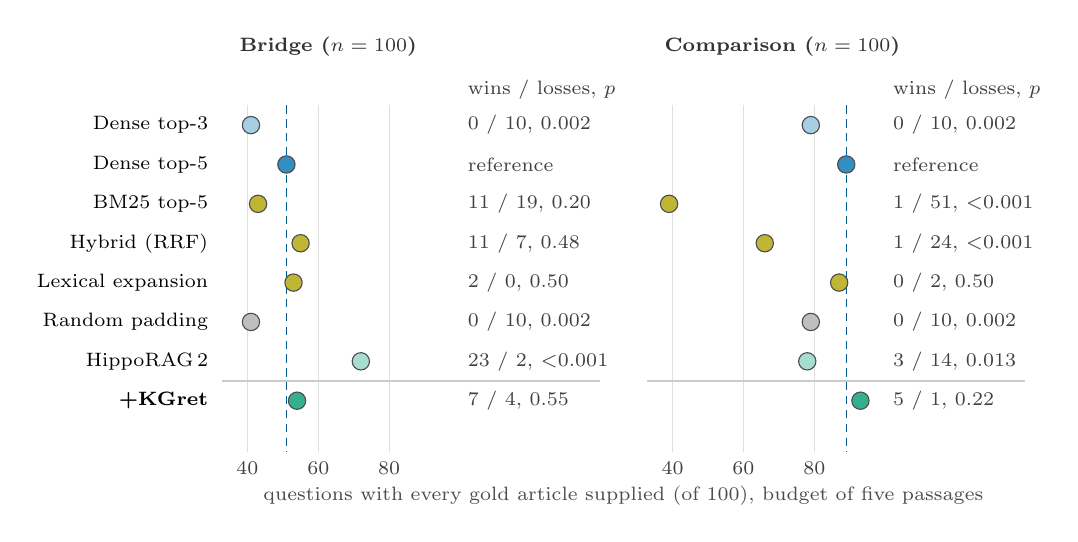
\begin{tikzpicture}[
  dot/.style  = {circle, inner sep=0pt, minimum size=2.2mm, draw=black!70, line width=0.4pt},
  row/.style  = {font=\scriptsize, anchor=east},
  num/.style  = {font=\scriptsize, anchor=west, text=black!75},
  tick/.style = {font=\scriptsize, text=black!75, below},
  ttl/.style  = {font=\scriptsize\bfseries, anchor=south west, text=black!80},
]
% A panel spans 35..95 questions at 0.045 cm per question; #1 is its x offset.
\def\xs{0.045}
\newcommand{\xof}[2]{#1+(#2-35)*\xs}
\newcommand{\axes}[3]{% offset, dense top-5 count, title
  \node[ttl] at (#1,0.75) {#3};
  \foreach \v in {40,60,80} {
    \draw[black!12] ({\xof{#1}{\v}},0.25) -- ({\xof{#1}{\v}},-4.15);
    \node[tick] at ({\xof{#1}{\v}},-4.15) {\v};
  }
  \draw[cText!80!black, densely dashed, line width=0.5pt]
    ({\xof{#1}{#2}},0.25) -- ({\xof{#1}{#2}},-4.15);
  \node[num, font=\scriptsize, text=black!75] at (#1+2.9,0.45) {wins / losses, $p$};
  \draw[black!20] (#1-0.1,-3.25) -- (#1+4.7,-3.25);}
\newcommand{\pt}[5]{% offset, y, count, fill, paired result
  \node[dot, fill=#4] at ({\xof{#1}{#3}},#2) {};
  \node[num] at (#1+2.9,#2) {#5};}

% Row labels
\foreach \y/\l in {0/Dense top-3, -0.5/Dense top-5, -1.0/BM25 top-5,
                   -1.5/Hybrid (RRF), -2.0/Lexical expansion,
                   -2.5/Random padding, -3.0/HippoRAG\,2, -3.5/\textbf{+KGret}}
  \node[row] at (-0.15,\y) {\l};

% Bridge
\axes{0}{51}{Bridge ($n=100$)}
\pt{0}{0}{41}{cText!35}{0 / 10, 0.002}
\pt{0}{-0.5}{51}{cText!80}{reference}
\pt{0}{-1.0}{43}{cAlt!80!black}{11 / 19, 0.20}
\pt{0}{-1.5}{55}{cAlt!80!black}{11 / 7, 0.48}
\pt{0}{-2.0}{53}{cAlt!80!black}{2 / 0, 0.50}
\pt{0}{-2.5}{41}{black!25}{0 / 10, 0.002}
\pt{0}{-3.0}{72}{cGraph!35}{23 / 2, $<$0.001}
\pt{0}{-3.5}{54}{cGraph!80}{7 / 4, 0.55}

% Comparison
\def\cx{5.4}
\axes{\cx}{89}{Comparison ($n=100$)}
\pt{\cx}{0}{79}{cText!35}{0 / 10, 0.002}
\pt{\cx}{-0.5}{89}{cText!80}{reference}
\pt{\cx}{-1.0}{39}{cAlt!80!black}{1 / 51, $<$0.001}
\pt{\cx}{-1.5}{66}{cAlt!80!black}{1 / 24, $<$0.001}
\pt{\cx}{-2.0}{87}{cAlt!80!black}{0 / 2, 0.50}
\pt{\cx}{-2.5}{79}{black!25}{0 / 10, 0.002}
\pt{\cx}{-3.0}{78}{cGraph!35}{3 / 14, 0.013}
\pt{\cx}{-3.5}{93}{cGraph!80}{5 / 1, 0.22}

\node[font=\scriptsize, text=black!70] at (5.0,-4.7)
  {questions with every gold article supplied (of 100), budget of five passages};
\end{tikzpicture}
\caption{Gold-evidence completeness at a budget of five passages on HotpotQA
bridge and comparison questions. Each dot counts the questions for which an
arm supplied every gold article, and the dashed line marks dense top-5. Wins
and losses are the questions an arm completes that dense top-5 does not, and
the reverse, with an exact McNemar $p$ before adjustment.}
\label{fig:rq1}
\end{figure*}


Our graph expansion barely changes how often the full gold evidence reaches
the generator. On the 100 bridge questions dense top-5 supplies both gold articles
for 51, and +KGret for 54 (Figure~\ref{fig:rq1}). +KGret completes seven
questions that dense top-5 does not and loses four that it does, which an
exact McNemar test cannot separate from chance ($p=0.55$ before adjustment).
Lexical expansion of the same query entities completes 53, and +KGret wins
five and loses four against it, so on bridge questions following graph edges
adds nothing measurable over matching the entity strings in chunk text. The
hybrid ranking completes 55 without any graph. The same pattern holds on the
comparison questions, where dense top-5 already completes 89 and +KGret
completes 93 (five wins, one loss, $p=0.22$). There +KGret also completes six
questions that lexical expansion misses and loses none ($p=0.031$ before
adjustment), but lexical expansion falls below dense top-5 on these questions,
so the difference reflects a weak control more than a gain from the graph.
BM25 and the hybrid lose ground on comparison questions, completing 39 and 66,
because predicate words such as ``contain gin'' outweigh the entity names in
BM25 scoring. Differences of a similar size are detectable with these 100
questions. Random padding, which spends the same two slots on arbitrary
chunks, loses ten bridge questions and wins none ($p=0.002$). Figure~\ref{fig:bridge} traces one of the seven bridge questions
+KGret recovers, which also shows the second slot going to an off-topic
article reached through a generic node.

HippoRAG\,2 behaves differently. At the same budget of five passages it
completes 72 bridge questions, winning 23 and losing 2 against dense top-5
($p<0.001$) and 23 to 5 against +KGret ($p<0.001$). Graph-based retrieval can
therefore recover bridge evidence that dense retrieval misses, which suggests
that the small effect of +KGret lies in how it links and ranks articles rather
than in graph retrieval as such. The gain does not carry over to
comparison questions, which name both entities. There HippoRAG\,2 completes 78
against 89 for dense top-5, losing 14 questions and winning 3 ($p=0.013$).

The answers follow the evidence. On the pre-specified primary outcome +KGret
and dense top-5 do not differ. Pooled over the five generators, exact match is
0.124 for +KGret and 0.120 for dense top-5, a paired difference of $+0.004$
(95\% CI $-0.012$ to $+0.022$), with 9 wins and 7 losses over 500
question--generator pairs and a Holm-adjusted $p$ of 1.00
(Table~\ref{tab:graph-bridge}). H1 is not supported. The secondary measures
give the same answer. Containment differs by $-0.002$ ($-0.038$ to $+0.038$)
and judge accuracy by $+0.004$ ($-0.034$ to $+0.044$), and the per-generator
results in Table~\ref{tab:graph-pergen} show no generator on which +KGret
gains more than 0.02 on any of the three. Dense top-5 itself gains 0.050 in
judge accuracy over dense top-3 ($p=0.029$ before adjustment and 0.29 after).
The data are therefore consistent with the earlier advantage of +KGret over
three-passage retrieval being an effect of the two extra passages, and the
interval for +KGret against dense top-5 stops just short of a gain of that
size. No non-graph arm at
the same budget beats dense top-5 either. Random padding, BM25, and dense
top-3 score 0.044 to 0.066 lower in judge accuracy, but none of these
differences survives the Holm adjustment ($p=0.29$ to 0.65).

HippoRAG\,2 is the only arm that changes the answers. It raises judge accuracy
from 0.634 to 0.794, a difference of $+0.160$ ($+0.092$ to $+0.232$; 86 wins,
6 losses; Holm-adjusted $p=0.002$), and containment by $+0.132$ ($+0.062$ to
$+0.206$; $p=0.013$), and it does so on every generator, by 0.15 in judge
accuracy for each of the three small models and by 0.18 and 0.17 for the two
strong ones. Its exact match moves by only $+0.010$ ($-0.020$ to
$+0.040$). The oracle arm shows how little room exact match leaves here. With
both gold articles supplied, pooled exact match is 0.216 while judge accuracy
is 0.938.

+KG, which adds the extracted triples to the dense top-3 prompt without
changing the passages, lowers exact match relative to dense top-3 from 0.120 to
0.090 (9 wins, 24 losses, $p=0.022$ before adjustment). Containment (0.494
against 0.478) and judge accuracy (0.590 against 0.584) do not change
measurably, and the loss in exact match comes mainly from Llama 4 Scout and
GPT-6 Luna (0.08 and 0.05), two of the generators that otherwise answer with a
short span. Injected facts thus
change how these generators word their answers more than whether the answers
are right.

The oracle and closed-book arms bound what retrieval can change. Judge accuracy
is 0.938 with both gold articles and 0.566 with no context, so dense top-5
recovers 18\% of that range and HippoRAG\,2 61\%. The closed-book floor differs
widely across generators, from 0.32 for Llama 4 Scout to 0.81 for Gemini 3.8
Flash. Qwen 3.8 Max used the whole output allowance and gave no answer on 18 of
its 100 closed-book questions. These count as incorrect, so its 0.64 is a lower
bound, and over the other 82 questions it scores 0.77. For Gemini 3.8 Flash and
GPT-6 Luna, accuracy with dense top-5 (0.62 and 0.66) is below closed-book
accuracy (0.81 and 0.69). On 26
bridge questions Gemini 3.8 Flash answers correctly without context but not
with dense top-5. On 24 of them dense top-5 did not supply both gold articles,
and in 25 the answer follows the instruction to say it does not know when the
context lacks the answer. Retrieval that misses evidence therefore costs this
generator answers it could otherwise give, which Section~\ref{sec:res-states}
returns to.

\subsection{Evidence deficit and the access/use split (RQ2)}
\label{sec:res-deficit}

\begin{table*}[!tbp]
\centering
\caption{HotpotQA comparison questions ($n=100$), five generators pooled (500
answers per row), with the columns of Table~\ref{tab:graph-bridge}.}
\label{tab:graph-comparison}
\footnotesize
\setlength{\tabcolsep}{3pt}
\resizebox{\textwidth}{!}{%
\begin{tabular}{@{}lccccccccc@{}}
\toprule
System & Complete. & EM & F1 & Contain. & Judge & $\Delta$EM & $p$ & $\Delta$Judge & $p$ \\
\midrule
Dense top-3 & 0.79 & 0.020 & 0.191 & 0.658 & 0.768 & 0.000 & 1.000 & $-$0.064 & 0.016 \\
 &  &  &  &  &  & {\scriptsize[$-$0.010, $+$0.010]} &  & {\scriptsize[$-$0.106, $-$0.028]} &  \\[1pt]
+KG & 0.79 & 0.012 & 0.180 & 0.676 & 0.774 & $-$0.008 & 1.000 & $-$0.058 & 0.227 \\
 &  &  &  &  &  & {\scriptsize[$-$0.020, $+$0.002]} &  & {\scriptsize[$-$0.106, $-$0.014]} &  \\[1pt]
Dense top-5 & 0.89 & 0.020 & 0.197 & 0.706 & 0.832 & ref. & -- & ref. & -- \\
BM25 top-5 & 0.39 & 0.006 & 0.137 & 0.456 & 0.510 & $-$0.014 & 1.000 & $-$0.322 & 0.002 \\
 &  &  &  &  &  & {\scriptsize[$-$0.030, $-$0.002]} &  & {\scriptsize[$-$0.412, $-$0.234]} &  \\[1pt]
Hybrid (RRF) & 0.66 & 0.014 & 0.182 & 0.622 & 0.698 & $-$0.006 & 1.000 & $-$0.134 & 0.006 \\
 &  &  &  &  &  & {\scriptsize[$-$0.014, 0.000]} &  & {\scriptsize[$-$0.208, $-$0.064]} &  \\[1pt]
Lexical expansion & 0.87 & 0.014 & 0.192 & 0.692 & 0.812 & $-$0.006 & 1.000 & $-$0.020 & 0.650 \\
 &  &  &  &  &  & {\scriptsize[$-$0.016, $+$0.002]} &  & {\scriptsize[$-$0.046, $+$0.002]} &  \\[1pt]
Random padding & 0.79 & 0.016 & 0.192 & 0.660 & 0.776 & $-$0.004 & 1.000 & $-$0.056 & 0.115 \\
 &  &  &  &  &  & {\scriptsize[$-$0.012, $+$0.004]} &  & {\scriptsize[$-$0.098, $-$0.018]} &  \\[1pt]
HippoRAG\,2 & 0.78 & 0.020 & 0.197 & 0.676 & 0.782 & 0.000 & 1.000 & $-$0.050 & 0.650 \\
 &  &  &  &  &  & {\scriptsize[$-$0.010, $+$0.008]} &  & {\scriptsize[$-$0.112, $+$0.010]} &  \\[1pt]
+KGret & 0.93 & 0.010 & 0.199 & 0.730 & 0.870 & $-$0.010 & 0.946 & $+$0.038 & 0.470 \\
 &  &  &  &  &  & {\scriptsize[$-$0.020, $-$0.002]} &  & {\scriptsize[$+$0.004, $+$0.078]} &  \\[1pt]
\midrule
Oracle & 1.00 & 0.022 & 0.219 & 0.740 & 0.894 & $+$0.002 & -- & $+$0.062 & -- \\
 &  &  &  &  &  & {\scriptsize[$-$0.004, $+$0.010]} &  & {\scriptsize[$+$0.002, $+$0.124]} &  \\[1pt]
Closed-book & -- & 0.004 & 0.143 & 0.670 & 0.756 & $-$0.016 & -- & $-$0.076 & -- \\
 &  &  &  &  &  & {\scriptsize[$-$0.036, 0.000]} &  & {\scriptsize[$-$0.150, 0.000]} &  \\[1pt]
\bottomrule
\end{tabular}}
\end{table*}

\begin{table*}[!tbp]
\centering
\caption{Decomposition (Eq.~\ref{eq:decomp}) of paired differences in exact
match and judge accuracy into access and use terms, five generators pooled,
with question-level cluster-bootstrap 95\% intervals. For +KG the access term
is zero by construction.}
\label{tab:decomp}
\footnotesize
\setlength{\tabcolsep}{4pt}
\resizebox{\textwidth}{!}{%
\begin{tabular}{@{}lcccccc@{}}
\toprule
& \multicolumn{3}{c}{Exact match} & \multicolumn{3}{c}{Judge accuracy} \\
\cmidrule(lr){2-4}\cmidrule(l){5-7}
Set & $\Delta$ & $\Delta_{\text{access}}$ & $\Delta_{\text{use}}$ & $\Delta$ & $\Delta_{\text{access}}$ & $\Delta_{\text{use}}$ \\
\midrule
\multicolumn{7}{@{}l}{\emph{+KGret minus dense top-5}} \\
Bridge & $+$0.004 & $+$0.003 & $+$0.001 & $+$0.004 & $+$0.017 & $-$0.013 \\
 & {\scriptsize[$-$0.012, $+$0.022]} & {\scriptsize[$-$0.003, $+$0.012]} & {\scriptsize[$-$0.018, $+$0.020]} & {\scriptsize[$-$0.034, $+$0.044]} & {\scriptsize[$-$0.020, $+$0.059]} & {\scriptsize[$-$0.052, $+$0.024]} \\
Comparison & $-$0.010 & 0.000 & $-$0.010 & $+$0.038 & $+$0.026 & $+$0.012 \\
 & {\scriptsize[$-$0.020, $-$0.002]} & {\scriptsize[$-$0.002, $+$0.002]} & {\scriptsize[$-$0.020, $-$0.002]} & {\scriptsize[$+$0.004, $+$0.078]} & {\scriptsize[0.000, $+$0.059]} & {\scriptsize[$-$0.013, $+$0.040]} \\
\addlinespace
\multicolumn{7}{@{}l}{\emph{+KG minus dense top-3}} \\
Bridge & $-$0.030 & 0 & $-$0.030 & $+$0.006 & 0 & $+$0.006 \\
 & {\scriptsize[$-$0.054, $-$0.006]} &  & {\scriptsize[$-$0.054, $-$0.006]} & {\scriptsize[$-$0.010, $+$0.022]} &  & {\scriptsize[$-$0.010, $+$0.022]} \\
Comparison & $-$0.008 & 0 & $-$0.008 & $+$0.006 & 0 & $+$0.006 \\
 & {\scriptsize[$-$0.022, $+$0.004]} &  & {\scriptsize[$-$0.022, $+$0.004]} & {\scriptsize[$-$0.016, $+$0.028]} &  & {\scriptsize[$-$0.016, $+$0.028]} \\
\addlinespace
\multicolumn{7}{@{}l}{\emph{HippoRAG\,2 minus dense top-5}} \\
Bridge & $+$0.010 & $+$0.020 & $-$0.010 & $+$0.160 & $+$0.120 & $+$0.040 \\
 & {\scriptsize[$-$0.020, $+$0.040]} & {\scriptsize[$+$0.004, $+$0.040]} & {\scriptsize[$-$0.041, $+$0.022]} & {\scriptsize[$+$0.092, $+$0.232]} & {\scriptsize[$+$0.061, $+$0.188]} & {\scriptsize[$-$0.011, $+$0.090]} \\
Comparison & 0.000 & 0.000 & 0.000 & $-$0.050 & $-$0.071 & $+$0.021 \\
 & {\scriptsize[$-$0.010, $+$0.008]} & {\scriptsize[$-$0.004, $+$0.006]} & {\scriptsize[$-$0.011, $+$0.010]} & {\scriptsize[$-$0.112, $+$0.010]} & {\scriptsize[$-$0.130, $-$0.022]} & {\scriptsize[$-$0.030, $+$0.068]} \\
\bottomrule
\end{tabular}}
\end{table*}

H2 is not supported. On comparison questions, where dense top-5 already
supplies both gold articles for 89 of 100, +KGret scores 0.038 higher in judge
accuracy ($+0.004$ to $+0.078$; 28 wins, 9 losses; $p=0.057$ before and 0.47
after adjustment) and 0.024 higher in containment ($-0.008$ to $+0.062$)
(Table~\ref{tab:graph-comparison}). On bridge questions the same differences
are $+0.004$ and $-0.002$. The bridge-minus-comparison contrast in the +KGret
effect is $-0.034$ for judge accuracy ($-0.090$ to $+0.018$) and $-0.020$ for
containment ($-0.070$ to $+0.030$). Both intervals include zero, and both
point estimates have the sign opposite to H2. In exact match the contrast is
$+0.014$ ($-0.004$ to $+0.034$), but on comparison questions exact match lies
between 0.00 and 0.06 for every generator and system, so this contrast
carries little information. Most of the small comparison difference lies in
the access term (0.026 of 0.038 in judge accuracy, Table~\ref{tab:decomp}),
which reflects the five questions on which +KGret supplies both articles and
dense top-5 does not, against one where the reverse holds. On bridge
questions the +KGret difference is too small to divide.

HippoRAG\,2 shows the pattern that H2 predicted for graph augmentation. It was
not part of the pre-specified hypothesis, so this analysis is exploratory. On
bridge questions, of its $+0.160$ gain in judge accuracy, $+0.120$ ($+0.061$
to $+0.188$) is access, the gain expected from moving questions into the
complete stratum at the per-stratum accuracy of dense top-5, and $+0.040$
($-0.011$ to $+0.090$) is use. The symmetric split, which does not depend on
which system is the reference, gives $+0.101$ ($+0.049$ to $+0.165$) for
access and $+0.059$ ($-0.001$ to $+0.119$) for use, so access carries most of
the gain under either weighting. On comparison questions, where it supplies
both articles for 11 fewer questions than dense top-5, its judge accuracy is
0.050 lower ($-0.112$ to $+0.010$; $p=0.13$ before adjustment), with an access
term of $-0.071$ ($-0.130$ to $-0.022$) and a symmetric access term of
$-0.068$. A graph retriever that changes which evidence arrives thus moves
answer accuracy through the access term, upward where it adds missing
evidence and, less certainly, downward where it displaces evidence that dense
retrieval had found. +KG changes no passages and its effect is confined to
the use term, where it lowers exact match on bridge questions by 0.030
($-0.054$ to $-0.006$) and leaves judge accuracy almost unchanged ($+0.006$,
$-0.010$ to $+0.022$).

\subsection{Mechanism test on graph-seeded questions}

These 50 questions were generated from entities shared by two papers in the
same graph that +KGret searches, and each names its linking entity. One
released question has an ellipsis in place of its reference answer and cannot
be scored, so results are reported on the remaining 49. They test whether the
mechanism works when the graph covers the intended relation; they are not
evidence about graph augmentation on questions written independently of the
graph. Their references are discursive, so answer containment is zero for
every arm and the judge's accuracy verdict is the outcome.

Even here the graph changes which papers reach the generator but not how
often the answer is right. +KGret supplies both gold papers for 36 of the 49
questions against 31 for dense top-5, yet pooled judge accuracy is 0.437
against 0.441 (21 wins, 22 losses; difference $-0.004$, 95\% CI $-0.086$ to
$+0.082$). +KG, with three passages and the extracted facts, scores 0.355,
0.086 below dense top-5 ($-0.180$ to 0.000; 20 wins, 41 losses, $p=0.088$
unadjusted); this set has no dense top-3 arm, so that difference mixes the
facts with the smaller passage budget. The attainable range is narrow. The
oracle arm reaches 0.563 and closed-book 0.371, from 0.04 for Gemini 3.8
Flash to 0.65 for GPT-6 Luna, which is above its 0.57 with dense top-5. On this
set the oracle arm is not
complete for every question. It passes the five chunks of the two gold papers
that rank highest for the question, and for 7 of the 49 questions all five
come from one paper. With one gold paper only (the partial-gold arm), accuracy
falls to 0.045, far below closed-book even though its F1 is higher (0.412
against 0.177). The answers we read suggest why. Many of these references state
general machine-learning knowledge that a generator can give unaided, while
with one paper it keeps to the context and reports that the other part is
missing, which the judge marks as wrong. These questions need both papers to
be answered from the context, not to be answered at all, which further limits
what this set can show about the graph.

\subsection{Multimodal augmentation and leakage (RQ3)}
\label{sec:res-mm}

\begin{table*}[!tbp]
\centering
\caption{SPIQA human-authored figure questions. Judge accuracy (primary),
pooled over four generators. Columns follow the filtering in
Figure~\ref{fig:funnel}, from the caption-flagged contrast set and the
screened primary set to the screened items whose answer does not occur in the
paper's retrievable text and, of those, the items no generator answers
closed-book. Caption arms share the text-only and closed-book answers of the
pixel run, which do not use the image path, and a dash marks an arm not run.
$\Delta$ is pixels minus text-only with a cluster-bootstrap 95\% interval, and
its $p$ is Holm-adjusted over the eight tests of the multimodal family.}
\label{tab:mm}
\footnotesize
\resizebox{\textwidth}{!}{%
\begin{tabular}{@{}lcccc@{}}
\toprule
Arm & Flagged ($n=132$) & Screened ($n=150$) & excl.\ text-recoverable ($n=135$) & excl.\ text and CB ($n=85$) \\
\midrule
Closed-book                & 0.100 & 0.187 & 0.200 & 0 \\
Text-only retrieval        & 0.241 & 0.285 & 0.293 & 0.194 \\
+multimodal (captions)     & -- & 0.333 & 0.344 & 0.235 \\
+multimodal (pixels, CLIP) & 0.278 & 0.358 & 0.365 & 0.256 \\
Oracle caption             & -- & 0.423 & 0.433 & 0.306 \\
Oracle image               & 0.680 & 0.643 & 0.630 & 0.568 \\
\midrule
$\Delta$ pixels -- text-only & $+0.038$ & $+0.073$ & $+0.072$ & $+0.062$ \\
95\% interval & $+0.002$ to $+0.078$ & $+0.038$ to $+0.110$ & $+0.037$ to $+0.111$ & $+0.024$ to $+0.106$ \\
Holm-adjusted $p$ & 0.28 & $<0.001$ & $<0.001$ & 0.019 \\
\bottomrule
\end{tabular}}
\end{table*}


Sending the top-ranked crop raises judge accuracy on the screened set from 0.285
to 0.358, a difference of $+0.073$ ($+0.038$ to $+0.110$, Holm-adjusted $p<0.001$;
Table~\ref{tab:mm}). Token F1 moves the same way, from 0.206 to 0.240. Neither
part of H3 is supported. We predicted a larger gain on caption-flagged items, but
there the difference is $+0.038$ ($+0.002$ to $+0.078$, Holm-adjusted $p=0.28$),
which is 0.035 below the screened set, although the interval for that contrast
includes zero ($-0.088$ to $+0.018$, Holm-adjusted $p=0.62$). We also predicted
that the gain would shrink when recoverable items are removed. Removing the 15
text-recoverable items leaves it at $+0.072$, and removing the 50 further items
that at least one generator answers closed-book leaves $+0.062$ ($+0.024$ to
$+0.106$, Holm-adjusted $p=0.019$) on the remaining 85. That is 0.012 below the
screened set, in the predicted direction, but the interval for the change includes
zero ($-0.045$ to $+0.021$, Holm-adjusted $p=0.62$). The gain differs between
generators, from $+0.027$ for Llama 4 Scout to $+0.107$ for GPT-6 Luna on the
screened set, and on the flagged set GPT-6 Luna is the one generator that loses
accuracy ($-0.015$). Captions of the top three crops raise accuracy on the
screened set by $+0.048$ ($+0.017$ to $+0.083$, Holm-adjusted $p=0.031$), but with
the adjudicated verdicts of Section~\ref{sec:judges} the adjusted $p$ becomes 0.06,
so we treat this gain as less secure than the gain from pixels.

Most of the gain the gold crop could bring is lost before the generator sees it.
CLIP ranks the gold crop first for 25 of the 150 screened questions (17\%) and 12
of the 132 flagged questions (9\%), and places it in the top five for 42 and 26.
Only the first crop is sent, so the pixel arm receives the gold crop for those 25
and 12 questions alone. Supplying the gold crop instead raises accuracy over
text-only by 0.358 ($+0.297$ to $+0.422$) on the screened set and 0.439 ($+0.367$
to $+0.511$) on the flagged set, so retrieved pixels recover 20\% and 9\% of those
gains. On the 25 screened questions where the top crop is gold, pixels reach 0.69
against 0.68 for the oracle image and 0.31 for text-only. On the other 125 they
reach 0.29 against 0.64 and 0.28, so a wrong crop neither helps nor visibly harms.
The flagged set shows the same pattern, with 0.73 against 0.75 and 0.27 on its 12
questions and 0.23 against 0.67 and 0.24 on the other 120. This split follows
retrieval and is therefore descriptive, since questions that CLIP ranks well may
differ in other ways. Figure reading is the other limit, because 36\% of screened
answers and 32\% of flagged answers remain wrong with the gold crop in hand. The
pixels of the gold crop carry more than its generated caption, with accuracy of
0.643 against 0.423 on the screened set ($+0.220$, $+0.162$ to $+0.280$).

PubLayNet shows the same mechanism at the floor of the scale. On its 35 pixel-only
questions text-only retrieval answers none of the 140 question--generator pairs
correctly and most replies decline. The oracle image reaches 0.293 and pixels
0.064 ($+0.064$, $0.000$ to $+0.150$, Holm-adjusted $p=0.62$). All 9 correct pixel
answers come from the 8 questions whose top crop is gold. Closed-book accuracy is
0.071, above text-only, so the floor on this corpus is low but not zero. With 35
model-authored questions this set supports
only the mechanism and not an estimate of the gain.

\note{The previous version's 25/34 versus $n=35$ denominator must not
reappear: every cell states its own $n$, and an unscorable item is named in
the caption.}

\subsection{Where answers come from (RQ4)}
\label{sec:res-states}

% RQ4: evidence states (Table~\ref{tab:states}) of every HotpotQA answer.
% Shares are from artifacts/runs/evidence_states_hotpotqa_{bridge,comparison}.csv,
% judge correctness and GPT-6.1 Sol sufficiency verdicts. Generated; do not edit by hand.
\begin{figure*}[t]
\centering
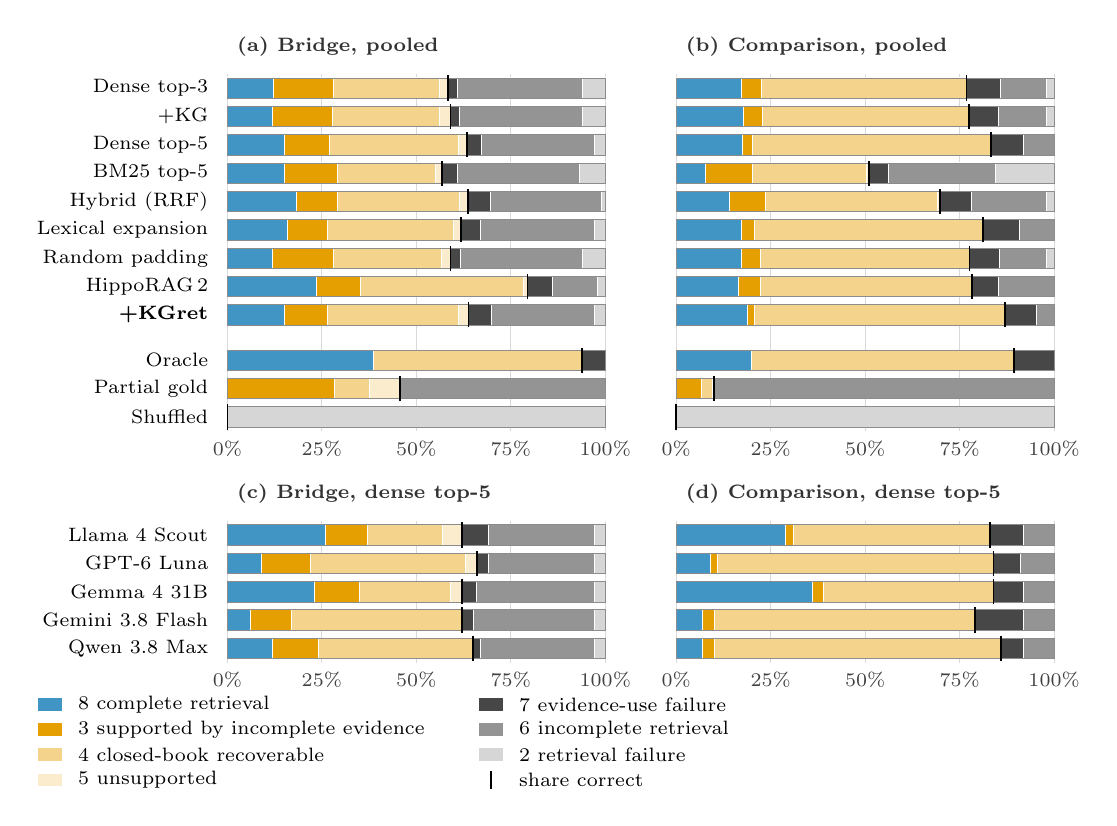
\begin{tikzpicture}[
  row/.style  = {font=\scriptsize, anchor=east},
  tick/.style = {font=\scriptsize, text=black!75, below},
  ttl/.style  = {font=\scriptsize\bfseries, anchor=south west, text=black!80},
  leg/.style  = {font=\scriptsize, anchor=west},
]
\node[ttl] at (0.000,0.280) {(a) Bridge, pooled};
\draw[black!15] (0.000,0.180) -- (0.000,-4.356);
\node[tick] at (0.000,-4.356) {0\%};
\draw[black!15] (1.200,0.180) -- (1.200,-4.356);
\node[tick] at (1.200,-4.356) {25\%};
\draw[black!15] (2.400,0.180) -- (2.400,-4.356);
\node[tick] at (2.400,-4.356) {50\%};
\draw[black!15] (3.600,0.180) -- (3.600,-4.356);
\node[tick] at (3.600,-4.356) {75\%};
\draw[black!15] (4.800,0.180) -- (4.800,-4.356);
\node[tick] at (4.800,-4.356) {100\%};
\node[ttl] at (5.700,0.280) {(b) Comparison, pooled};
\draw[black!15] (5.700,0.180) -- (5.700,-4.356);
\node[tick] at (5.700,-4.356) {0\%};
\draw[black!15] (6.900,0.180) -- (6.900,-4.356);
\node[tick] at (6.900,-4.356) {25\%};
\draw[black!15] (8.100,0.180) -- (8.100,-4.356);
\node[tick] at (8.100,-4.356) {50\%};
\draw[black!15] (9.300,0.180) -- (9.300,-4.356);
\node[tick] at (9.300,-4.356) {75\%};
\draw[black!15] (10.500,0.180) -- (10.500,-4.356);
\node[tick] at (10.500,-4.356) {100\%};
\filldraw[fill=cCredit!75, draw=white, line width=0.3pt] (0.000,-0.130) rectangle (0.586,0.130);
\filldraw[fill=cNotCredit, draw=white, line width=0.3pt] (0.586,-0.130) rectangle (1.344,0.130);
\filldraw[fill=cNotCredit!45, draw=white, line width=0.3pt] (1.344,-0.130) rectangle (2.688,0.130);
\filldraw[fill=cNotCredit!20, draw=white, line width=0.3pt] (2.688,-0.130) rectangle (2.803,0.130);
\filldraw[fill=black!72, draw=white, line width=0.3pt] (2.803,-0.130) rectangle (2.928,0.130);
\filldraw[fill=black!42, draw=white, line width=0.3pt] (2.928,-0.130) rectangle (4.512,0.130);
\filldraw[fill=black!16, draw=white, line width=0.3pt] (4.512,-0.130) rectangle (4.800,0.130);
\draw[black!45, line width=0.25pt] (0.000,-0.130) rectangle (4.800,0.130);
\draw[black, line width=0.6pt] (2.803,-0.160) -- (2.803,0.160);
\node[row] at (-0.120,0.000) {Dense top-3};
\filldraw[fill=cCredit!75, draw=white, line width=0.3pt] (5.700,-0.130) rectangle (6.526,0.130);
\filldraw[fill=cNotCredit, draw=white, line width=0.3pt] (6.526,-0.130) rectangle (6.785,0.130);
\filldraw[fill=cNotCredit!45, draw=white, line width=0.3pt] (6.785,-0.130) rectangle (9.386,0.130);
\filldraw[fill=black!72, draw=white, line width=0.3pt] (9.386,-0.130) rectangle (9.818,0.130);
\filldraw[fill=black!42, draw=white, line width=0.3pt] (9.818,-0.130) rectangle (10.404,0.130);
\filldraw[fill=black!16, draw=white, line width=0.3pt] (10.404,-0.130) rectangle (10.500,0.130);
\draw[black!45, line width=0.25pt] (5.700,-0.130) rectangle (10.500,0.130);
\draw[black, line width=0.6pt] (9.386,-0.160) -- (9.386,0.160);
\filldraw[fill=cCredit!75, draw=white, line width=0.3pt] (0.000,-0.490) rectangle (0.566,-0.230);
\filldraw[fill=cNotCredit, draw=white, line width=0.3pt] (0.566,-0.490) rectangle (1.334,-0.230);
\filldraw[fill=cNotCredit!45, draw=white, line width=0.3pt] (1.334,-0.490) rectangle (2.698,-0.230);
\filldraw[fill=cNotCredit!20, draw=white, line width=0.3pt] (2.698,-0.490) rectangle (2.832,-0.230);
\filldraw[fill=black!72, draw=white, line width=0.3pt] (2.832,-0.490) rectangle (2.947,-0.230);
\filldraw[fill=black!42, draw=white, line width=0.3pt] (2.947,-0.490) rectangle (4.512,-0.230);
\filldraw[fill=black!16, draw=white, line width=0.3pt] (4.512,-0.490) rectangle (4.800,-0.230);
\draw[black!45, line width=0.25pt] (0.000,-0.490) rectangle (4.800,-0.230);
\draw[black, line width=0.6pt] (2.832,-0.520) -- (2.832,-0.200);
\node[row] at (-0.120,-0.360) {+KG};
\filldraw[fill=cCredit!75, draw=white, line width=0.3pt] (5.700,-0.490) rectangle (6.554,-0.230);
\filldraw[fill=cNotCredit, draw=white, line width=0.3pt] (6.554,-0.490) rectangle (6.794,-0.230);
\filldraw[fill=cNotCredit!45, draw=white, line width=0.3pt] (6.794,-0.490) rectangle (9.415,-0.230);
\filldraw[fill=black!72, draw=white, line width=0.3pt] (9.415,-0.490) rectangle (9.790,-0.230);
\filldraw[fill=black!42, draw=white, line width=0.3pt] (9.790,-0.490) rectangle (10.404,-0.230);
\filldraw[fill=black!16, draw=white, line width=0.3pt] (10.404,-0.490) rectangle (10.500,-0.230);
\draw[black!45, line width=0.25pt] (5.700,-0.490) rectangle (10.500,-0.230);
\draw[black, line width=0.6pt] (9.415,-0.520) -- (9.415,-0.200);
\filldraw[fill=cCredit!75, draw=white, line width=0.3pt] (0.000,-0.850) rectangle (0.730,-0.590);
\filldraw[fill=cNotCredit, draw=white, line width=0.3pt] (0.730,-0.850) rectangle (1.296,-0.590);
\filldraw[fill=cNotCredit!45, draw=white, line width=0.3pt] (1.296,-0.850) rectangle (2.938,-0.590);
\filldraw[fill=cNotCredit!20, draw=white, line width=0.3pt] (2.938,-0.850) rectangle (3.043,-0.590);
\filldraw[fill=black!72, draw=white, line width=0.3pt] (3.043,-0.850) rectangle (3.226,-0.590);
\filldraw[fill=black!42, draw=white, line width=0.3pt] (3.226,-0.850) rectangle (4.656,-0.590);
\filldraw[fill=black!16, draw=white, line width=0.3pt] (4.656,-0.850) rectangle (4.800,-0.590);
\draw[black!45, line width=0.25pt] (0.000,-0.850) rectangle (4.800,-0.590);
\draw[black, line width=0.6pt] (3.043,-0.880) -- (3.043,-0.560);
\node[row] at (-0.120,-0.720) {Dense top-5};
\filldraw[fill=cCredit!75, draw=white, line width=0.3pt] (5.700,-0.850) rectangle (6.545,-0.590);
\filldraw[fill=cNotCredit, draw=white, line width=0.3pt] (6.545,-0.850) rectangle (6.670,-0.590);
\filldraw[fill=cNotCredit!45, draw=white, line width=0.3pt] (6.670,-0.850) rectangle (9.694,-0.590);
\filldraw[fill=black!72, draw=white, line width=0.3pt] (9.694,-0.850) rectangle (10.106,-0.590);
\filldraw[fill=black!42, draw=white, line width=0.3pt] (10.106,-0.850) rectangle (10.500,-0.590);
\draw[black!45, line width=0.25pt] (5.700,-0.850) rectangle (10.500,-0.590);
\draw[black, line width=0.6pt] (9.694,-0.880) -- (9.694,-0.560);
\filldraw[fill=cCredit!75, draw=white, line width=0.3pt] (0.000,-1.210) rectangle (0.720,-0.950);
\filldraw[fill=cNotCredit, draw=white, line width=0.3pt] (0.720,-1.210) rectangle (1.392,-0.950);
\filldraw[fill=cNotCredit!45, draw=white, line width=0.3pt] (1.392,-1.210) rectangle (2.640,-0.950);
\filldraw[fill=cNotCredit!20, draw=white, line width=0.3pt] (2.640,-1.210) rectangle (2.726,-0.950);
\filldraw[fill=black!72, draw=white, line width=0.3pt] (2.726,-1.210) rectangle (2.928,-0.950);
\filldraw[fill=black!42, draw=white, line width=0.3pt] (2.928,-1.210) rectangle (4.474,-0.950);
\filldraw[fill=black!16, draw=white, line width=0.3pt] (4.474,-1.210) rectangle (4.800,-0.950);
\draw[black!45, line width=0.25pt] (0.000,-1.210) rectangle (4.800,-0.950);
\draw[black, line width=0.6pt] (2.726,-1.240) -- (2.726,-0.920);
\node[row] at (-0.120,-1.080) {BM25 top-5};
\filldraw[fill=cCredit!75, draw=white, line width=0.3pt] (5.700,-1.210) rectangle (6.074,-0.950);
\filldraw[fill=cNotCredit, draw=white, line width=0.3pt] (6.074,-1.210) rectangle (6.670,-0.950);
\filldraw[fill=cNotCredit!45, draw=white, line width=0.3pt] (6.670,-1.210) rectangle (8.110,-0.950);
\filldraw[fill=cNotCredit!20, draw=white, line width=0.3pt] (8.110,-1.210) rectangle (8.148,-0.950);
\filldraw[fill=black!72, draw=white, line width=0.3pt] (8.148,-1.210) rectangle (8.398,-0.950);
\filldraw[fill=black!42, draw=white, line width=0.3pt] (8.398,-1.210) rectangle (9.751,-0.950);
\filldraw[fill=black!16, draw=white, line width=0.3pt] (9.751,-1.210) rectangle (10.500,-0.950);
\draw[black!45, line width=0.25pt] (5.700,-1.210) rectangle (10.500,-0.950);
\draw[black, line width=0.6pt] (8.148,-1.240) -- (8.148,-0.920);
\filldraw[fill=cCredit!75, draw=white, line width=0.3pt] (0.000,-1.570) rectangle (0.883,-1.310);
\filldraw[fill=cNotCredit, draw=white, line width=0.3pt] (0.883,-1.570) rectangle (1.392,-1.310);
\filldraw[fill=cNotCredit!45, draw=white, line width=0.3pt] (1.392,-1.570) rectangle (2.947,-1.310);
\filldraw[fill=cNotCredit!20, draw=white, line width=0.3pt] (2.947,-1.570) rectangle (3.053,-1.310);
\filldraw[fill=black!72, draw=white, line width=0.3pt] (3.053,-1.570) rectangle (3.341,-1.310);
\filldraw[fill=black!42, draw=white, line width=0.3pt] (3.341,-1.570) rectangle (4.752,-1.310);
\filldraw[fill=black!16, draw=white, line width=0.3pt] (4.752,-1.570) rectangle (4.800,-1.310);
\draw[black!45, line width=0.25pt] (0.000,-1.570) rectangle (4.800,-1.310);
\draw[black, line width=0.6pt] (3.053,-1.600) -- (3.053,-1.280);
\node[row] at (-0.120,-1.440) {Hybrid (RRF)};
\filldraw[fill=cCredit!75, draw=white, line width=0.3pt] (5.700,-1.570) rectangle (6.382,-1.310);
\filldraw[fill=cNotCredit, draw=white, line width=0.3pt] (6.382,-1.570) rectangle (6.833,-1.310);
\filldraw[fill=cNotCredit!45, draw=white, line width=0.3pt] (6.833,-1.570) rectangle (9.022,-1.310);
\filldraw[fill=cNotCredit!20, draw=white, line width=0.3pt] (9.022,-1.570) rectangle (9.050,-1.310);
\filldraw[fill=black!72, draw=white, line width=0.3pt] (9.050,-1.570) rectangle (9.444,-1.310);
\filldraw[fill=black!42, draw=white, line width=0.3pt] (9.444,-1.570) rectangle (10.404,-1.310);
\filldraw[fill=black!16, draw=white, line width=0.3pt] (10.404,-1.570) rectangle (10.500,-1.310);
\draw[black!45, line width=0.25pt] (5.700,-1.570) rectangle (10.500,-1.310);
\draw[black, line width=0.6pt] (9.050,-1.600) -- (9.050,-1.280);
\filldraw[fill=cCredit!75, draw=white, line width=0.3pt] (0.000,-1.930) rectangle (0.758,-1.670);
\filldraw[fill=cNotCredit, draw=white, line width=0.3pt] (0.758,-1.930) rectangle (1.277,-1.670);
\filldraw[fill=cNotCredit!45, draw=white, line width=0.3pt] (1.277,-1.930) rectangle (2.870,-1.670);
\filldraw[fill=cNotCredit!20, draw=white, line width=0.3pt] (2.870,-1.930) rectangle (2.966,-1.670);
\filldraw[fill=black!72, draw=white, line width=0.3pt] (2.966,-1.930) rectangle (3.216,-1.670);
\filldraw[fill=black!42, draw=white, line width=0.3pt] (3.216,-1.930) rectangle (4.656,-1.670);
\filldraw[fill=black!16, draw=white, line width=0.3pt] (4.656,-1.930) rectangle (4.800,-1.670);
\draw[black!45, line width=0.25pt] (0.000,-1.930) rectangle (4.800,-1.670);
\draw[black, line width=0.6pt] (2.966,-1.960) -- (2.966,-1.640);
\node[row] at (-0.120,-1.800) {Lexical expansion};
\filldraw[fill=cCredit!75, draw=white, line width=0.3pt] (5.700,-1.930) rectangle (6.526,-1.670);
\filldraw[fill=cNotCredit, draw=white, line width=0.3pt] (6.526,-1.930) rectangle (6.698,-1.670);
\filldraw[fill=cNotCredit!45, draw=white, line width=0.3pt] (6.698,-1.930) rectangle (9.598,-1.670);
\filldraw[fill=black!72, draw=white, line width=0.3pt] (9.598,-1.930) rectangle (10.058,-1.670);
\filldraw[fill=black!42, draw=white, line width=0.3pt] (10.058,-1.930) rectangle (10.500,-1.670);
\draw[black!45, line width=0.25pt] (5.700,-1.930) rectangle (10.500,-1.670);
\draw[black, line width=0.6pt] (9.598,-1.960) -- (9.598,-1.640);
\filldraw[fill=cCredit!75, draw=white, line width=0.3pt] (0.000,-2.290) rectangle (0.576,-2.030);
\filldraw[fill=cNotCredit, draw=white, line width=0.3pt] (0.576,-2.290) rectangle (1.344,-2.030);
\filldraw[fill=cNotCredit!45, draw=white, line width=0.3pt] (1.344,-2.290) rectangle (2.717,-2.030);
\filldraw[fill=cNotCredit!20, draw=white, line width=0.3pt] (2.717,-2.290) rectangle (2.832,-2.030);
\filldraw[fill=black!72, draw=white, line width=0.3pt] (2.832,-2.290) rectangle (2.957,-2.030);
\filldraw[fill=black!42, draw=white, line width=0.3pt] (2.957,-2.290) rectangle (4.512,-2.030);
\filldraw[fill=black!16, draw=white, line width=0.3pt] (4.512,-2.290) rectangle (4.800,-2.030);
\draw[black!45, line width=0.25pt] (0.000,-2.290) rectangle (4.800,-2.030);
\draw[black, line width=0.6pt] (2.832,-2.320) -- (2.832,-2.000);
\node[row] at (-0.120,-2.160) {Random padding};
\filldraw[fill=cCredit!75, draw=white, line width=0.3pt] (5.700,-2.290) rectangle (6.526,-2.030);
\filldraw[fill=cNotCredit, draw=white, line width=0.3pt] (6.526,-2.290) rectangle (6.766,-2.030);
\filldraw[fill=cNotCredit!45, draw=white, line width=0.3pt] (6.766,-2.290) rectangle (9.425,-2.030);
\filldraw[fill=black!72, draw=white, line width=0.3pt] (9.425,-2.290) rectangle (9.799,-2.030);
\filldraw[fill=black!42, draw=white, line width=0.3pt] (9.799,-2.290) rectangle (10.404,-2.030);
\filldraw[fill=black!16, draw=white, line width=0.3pt] (10.404,-2.290) rectangle (10.500,-2.030);
\draw[black!45, line width=0.25pt] (5.700,-2.290) rectangle (10.500,-2.030);
\draw[black, line width=0.6pt] (9.425,-2.320) -- (9.425,-2.000);
\filldraw[fill=cCredit!75, draw=white, line width=0.3pt] (0.000,-2.650) rectangle (1.133,-2.390);
\filldraw[fill=cNotCredit, draw=white, line width=0.3pt] (1.133,-2.650) rectangle (1.690,-2.390);
\filldraw[fill=cNotCredit!45, draw=white, line width=0.3pt] (1.690,-2.650) rectangle (3.763,-2.390);
\filldraw[fill=cNotCredit!20, draw=white, line width=0.3pt] (3.763,-2.650) rectangle (3.811,-2.390);
\filldraw[fill=black!72, draw=white, line width=0.3pt] (3.811,-2.650) rectangle (4.128,-2.390);
\filldraw[fill=black!42, draw=white, line width=0.3pt] (4.128,-2.650) rectangle (4.704,-2.390);
\filldraw[fill=black!16, draw=white, line width=0.3pt] (4.704,-2.650) rectangle (4.800,-2.390);
\draw[black!45, line width=0.25pt] (0.000,-2.650) rectangle (4.800,-2.390);
\draw[black, line width=0.6pt] (3.811,-2.680) -- (3.811,-2.360);
\node[row] at (-0.120,-2.520) {HippoRAG\,2};
\filldraw[fill=cCredit!75, draw=white, line width=0.3pt] (5.700,-2.650) rectangle (6.487,-2.390);
\filldraw[fill=cNotCredit, draw=white, line width=0.3pt] (6.487,-2.650) rectangle (6.775,-2.390);
\filldraw[fill=cNotCredit!45, draw=white, line width=0.3pt] (6.775,-2.650) rectangle (9.444,-2.390);
\filldraw[fill=cNotCredit!20, draw=white, line width=0.3pt] (9.444,-2.650) rectangle (9.454,-2.390);
\filldraw[fill=black!72, draw=white, line width=0.3pt] (9.454,-2.650) rectangle (9.790,-2.390);
\filldraw[fill=black!42, draw=white, line width=0.3pt] (9.790,-2.650) rectangle (10.500,-2.390);
\draw[black!45, line width=0.25pt] (5.700,-2.650) rectangle (10.500,-2.390);
\draw[black, line width=0.6pt] (9.454,-2.680) -- (9.454,-2.360);
\filldraw[fill=cCredit!75, draw=white, line width=0.3pt] (0.000,-3.010) rectangle (0.730,-2.750);
\filldraw[fill=cNotCredit, draw=white, line width=0.3pt] (0.730,-3.010) rectangle (1.277,-2.750);
\filldraw[fill=cNotCredit!45, draw=white, line width=0.3pt] (1.277,-3.010) rectangle (2.938,-2.750);
\filldraw[fill=cNotCredit!20, draw=white, line width=0.3pt] (2.938,-3.010) rectangle (3.062,-2.750);
\filldraw[fill=black!72, draw=white, line width=0.3pt] (3.062,-3.010) rectangle (3.350,-2.750);
\filldraw[fill=black!42, draw=white, line width=0.3pt] (3.350,-3.010) rectangle (4.656,-2.750);
\filldraw[fill=black!16, draw=white, line width=0.3pt] (4.656,-3.010) rectangle (4.800,-2.750);
\draw[black!45, line width=0.25pt] (0.000,-3.010) rectangle (4.800,-2.750);
\draw[black, line width=0.6pt] (3.062,-3.040) -- (3.062,-2.720);
\node[row] at (-0.120,-2.880) {\textbf{+KGret}};
\filldraw[fill=cCredit!75, draw=white, line width=0.3pt] (5.700,-3.010) rectangle (6.602,-2.750);
\filldraw[fill=cNotCredit, draw=white, line width=0.3pt] (6.602,-3.010) rectangle (6.698,-2.750);
\filldraw[fill=cNotCredit!45, draw=white, line width=0.3pt] (6.698,-3.010) rectangle (9.876,-2.750);
\filldraw[fill=black!72, draw=white, line width=0.3pt] (9.876,-3.010) rectangle (10.279,-2.750);
\filldraw[fill=black!42, draw=white, line width=0.3pt] (10.279,-3.010) rectangle (10.500,-2.750);
\draw[black!45, line width=0.25pt] (5.700,-3.010) rectangle (10.500,-2.750);
\draw[black, line width=0.6pt] (9.876,-3.040) -- (9.876,-2.720);
\filldraw[fill=cCredit!75, draw=white, line width=0.3pt] (0.000,-3.586) rectangle (1.853,-3.326);
\filldraw[fill=cNotCredit!45, draw=white, line width=0.3pt] (1.853,-3.586) rectangle (4.502,-3.326);
\filldraw[fill=black!72, draw=white, line width=0.3pt] (4.502,-3.586) rectangle (4.800,-3.326);
\draw[black!45, line width=0.25pt] (0.000,-3.586) rectangle (4.800,-3.326);
\draw[black, line width=0.6pt] (4.502,-3.616) -- (4.502,-3.296);
\node[row] at (-0.120,-3.456) {Oracle};
\filldraw[fill=cCredit!75, draw=white, line width=0.3pt] (5.700,-3.586) rectangle (6.660,-3.326);
\filldraw[fill=cNotCredit!45, draw=white, line width=0.3pt] (6.660,-3.586) rectangle (9.991,-3.326);
\filldraw[fill=black!72, draw=white, line width=0.3pt] (9.991,-3.586) rectangle (10.500,-3.326);
\draw[black!45, line width=0.25pt] (5.700,-3.586) rectangle (10.500,-3.326);
\draw[black, line width=0.6pt] (9.991,-3.616) -- (9.991,-3.296);
\filldraw[fill=cNotCredit, draw=white, line width=0.3pt] (0.000,-3.946) rectangle (1.354,-3.686);
\filldraw[fill=cNotCredit!45, draw=white, line width=0.3pt] (1.354,-3.946) rectangle (1.805,-3.686);
\filldraw[fill=cNotCredit!20, draw=white, line width=0.3pt] (1.805,-3.946) rectangle (2.189,-3.686);
\filldraw[fill=black!42, draw=white, line width=0.3pt] (2.189,-3.946) rectangle (4.800,-3.686);
\draw[black!45, line width=0.25pt] (0.000,-3.946) rectangle (4.800,-3.686);
\draw[black, line width=0.6pt] (2.189,-3.976) -- (2.189,-3.656);
\node[row] at (-0.120,-3.816) {Partial gold};
\filldraw[fill=cNotCredit, draw=white, line width=0.3pt] (5.700,-3.946) rectangle (6.026,-3.686);
\filldraw[fill=cNotCredit!45, draw=white, line width=0.3pt] (6.026,-3.946) rectangle (6.161,-3.686);
\filldraw[fill=cNotCredit!20, draw=white, line width=0.3pt] (6.161,-3.946) rectangle (6.180,-3.686);
\filldraw[fill=black!42, draw=white, line width=0.3pt] (6.180,-3.946) rectangle (10.500,-3.686);
\draw[black!45, line width=0.25pt] (5.700,-3.946) rectangle (10.500,-3.686);
\draw[black, line width=0.6pt] (6.180,-3.976) -- (6.180,-3.656);
\filldraw[fill=black!16, draw=white, line width=0.3pt] (0.000,-4.306) rectangle (4.800,-4.046);
\draw[black!45, line width=0.25pt] (0.000,-4.306) rectangle (4.800,-4.046);
\draw[black, line width=0.6pt] (0.000,-4.336) -- (0.000,-4.016);
\node[row] at (-0.120,-4.176) {Shuffled};
\filldraw[fill=black!16, draw=white, line width=0.3pt] (5.700,-4.306) rectangle (10.500,-4.046);
\draw[black!45, line width=0.25pt] (5.700,-4.306) rectangle (10.500,-4.046);
\draw[black, line width=0.6pt] (5.700,-4.336) -- (5.700,-4.016);
\node[ttl] at (0.000,-5.396) {(c) Bridge, dense top-5};
\draw[black!15] (0.000,-5.496) -- (0.000,-7.296);
\node[tick] at (0.000,-7.296) {0\%};
\draw[black!15] (1.200,-5.496) -- (1.200,-7.296);
\node[tick] at (1.200,-7.296) {25\%};
\draw[black!15] (2.400,-5.496) -- (2.400,-7.296);
\node[tick] at (2.400,-7.296) {50\%};
\draw[black!15] (3.600,-5.496) -- (3.600,-7.296);
\node[tick] at (3.600,-7.296) {75\%};
\draw[black!15] (4.800,-5.496) -- (4.800,-7.296);
\node[tick] at (4.800,-7.296) {100\%};
\filldraw[fill=cCredit!75, draw=white, line width=0.3pt] (0.000,-5.806) rectangle (1.248,-5.546);
\filldraw[fill=cNotCredit, draw=white, line width=0.3pt] (1.248,-5.806) rectangle (1.776,-5.546);
\filldraw[fill=cNotCredit!45, draw=white, line width=0.3pt] (1.776,-5.806) rectangle (2.736,-5.546);
\filldraw[fill=cNotCredit!20, draw=white, line width=0.3pt] (2.736,-5.806) rectangle (2.976,-5.546);
\filldraw[fill=black!72, draw=white, line width=0.3pt] (2.976,-5.806) rectangle (3.312,-5.546);
\filldraw[fill=black!42, draw=white, line width=0.3pt] (3.312,-5.806) rectangle (4.656,-5.546);
\filldraw[fill=black!16, draw=white, line width=0.3pt] (4.656,-5.806) rectangle (4.800,-5.546);
\draw[black!45, line width=0.25pt] (0.000,-5.806) rectangle (4.800,-5.546);
\draw[black, line width=0.6pt] (2.976,-5.836) -- (2.976,-5.516);
\node[row] at (-0.120,-5.676) {Llama 4 Scout};
\filldraw[fill=cCredit!75, draw=white, line width=0.3pt] (0.000,-6.166) rectangle (0.432,-5.906);
\filldraw[fill=cNotCredit, draw=white, line width=0.3pt] (0.432,-6.166) rectangle (1.056,-5.906);
\filldraw[fill=cNotCredit!45, draw=white, line width=0.3pt] (1.056,-6.166) rectangle (3.024,-5.906);
\filldraw[fill=cNotCredit!20, draw=white, line width=0.3pt] (3.024,-6.166) rectangle (3.168,-5.906);
\filldraw[fill=black!72, draw=white, line width=0.3pt] (3.168,-6.166) rectangle (3.312,-5.906);
\filldraw[fill=black!42, draw=white, line width=0.3pt] (3.312,-6.166) rectangle (4.656,-5.906);
\filldraw[fill=black!16, draw=white, line width=0.3pt] (4.656,-6.166) rectangle (4.800,-5.906);
\draw[black!45, line width=0.25pt] (0.000,-6.166) rectangle (4.800,-5.906);
\draw[black, line width=0.6pt] (3.168,-6.196) -- (3.168,-5.876);
\node[row] at (-0.120,-6.036) {GPT-6 Luna};
\filldraw[fill=cCredit!75, draw=white, line width=0.3pt] (0.000,-6.526) rectangle (1.104,-6.266);
\filldraw[fill=cNotCredit, draw=white, line width=0.3pt] (1.104,-6.526) rectangle (1.680,-6.266);
\filldraw[fill=cNotCredit!45, draw=white, line width=0.3pt] (1.680,-6.526) rectangle (2.832,-6.266);
\filldraw[fill=cNotCredit!20, draw=white, line width=0.3pt] (2.832,-6.526) rectangle (2.976,-6.266);
\filldraw[fill=black!72, draw=white, line width=0.3pt] (2.976,-6.526) rectangle (3.168,-6.266);
\filldraw[fill=black!42, draw=white, line width=0.3pt] (3.168,-6.526) rectangle (4.656,-6.266);
\filldraw[fill=black!16, draw=white, line width=0.3pt] (4.656,-6.526) rectangle (4.800,-6.266);
\draw[black!45, line width=0.25pt] (0.000,-6.526) rectangle (4.800,-6.266);
\draw[black, line width=0.6pt] (2.976,-6.556) -- (2.976,-6.236);
\node[row] at (-0.120,-6.396) {Gemma 4 31B};
\filldraw[fill=cCredit!75, draw=white, line width=0.3pt] (0.000,-6.886) rectangle (0.288,-6.626);
\filldraw[fill=cNotCredit, draw=white, line width=0.3pt] (0.288,-6.886) rectangle (0.816,-6.626);
\filldraw[fill=cNotCredit!45, draw=white, line width=0.3pt] (0.816,-6.886) rectangle (2.976,-6.626);
\filldraw[fill=black!72, draw=white, line width=0.3pt] (2.976,-6.886) rectangle (3.120,-6.626);
\filldraw[fill=black!42, draw=white, line width=0.3pt] (3.120,-6.886) rectangle (4.656,-6.626);
\filldraw[fill=black!16, draw=white, line width=0.3pt] (4.656,-6.886) rectangle (4.800,-6.626);
\draw[black!45, line width=0.25pt] (0.000,-6.886) rectangle (4.800,-6.626);
\draw[black, line width=0.6pt] (2.976,-6.916) -- (2.976,-6.596);
\node[row] at (-0.120,-6.756) {Gemini 3.8 Flash};
\filldraw[fill=cCredit!75, draw=white, line width=0.3pt] (0.000,-7.246) rectangle (0.576,-6.986);
\filldraw[fill=cNotCredit, draw=white, line width=0.3pt] (0.576,-7.246) rectangle (1.152,-6.986);
\filldraw[fill=cNotCredit!45, draw=white, line width=0.3pt] (1.152,-7.246) rectangle (3.120,-6.986);
\filldraw[fill=black!72, draw=white, line width=0.3pt] (3.120,-7.246) rectangle (3.216,-6.986);
\filldraw[fill=black!42, draw=white, line width=0.3pt] (3.216,-7.246) rectangle (4.656,-6.986);
\filldraw[fill=black!16, draw=white, line width=0.3pt] (4.656,-7.246) rectangle (4.800,-6.986);
\draw[black!45, line width=0.25pt] (0.000,-7.246) rectangle (4.800,-6.986);
\draw[black, line width=0.6pt] (3.120,-7.276) -- (3.120,-6.956);
\node[row] at (-0.120,-7.116) {Qwen 3.8 Max};
\node[ttl] at (5.700,-5.396) {(d) Comparison, dense top-5};
\draw[black!15] (5.700,-5.496) -- (5.700,-7.296);
\node[tick] at (5.700,-7.296) {0\%};
\draw[black!15] (6.900,-5.496) -- (6.900,-7.296);
\node[tick] at (6.900,-7.296) {25\%};
\draw[black!15] (8.100,-5.496) -- (8.100,-7.296);
\node[tick] at (8.100,-7.296) {50\%};
\draw[black!15] (9.300,-5.496) -- (9.300,-7.296);
\node[tick] at (9.300,-7.296) {75\%};
\draw[black!15] (10.500,-5.496) -- (10.500,-7.296);
\node[tick] at (10.500,-7.296) {100\%};
\filldraw[fill=cCredit!75, draw=white, line width=0.3pt] (5.700,-5.806) rectangle (7.092,-5.546);
\filldraw[fill=cNotCredit, draw=white, line width=0.3pt] (7.092,-5.806) rectangle (7.188,-5.546);
\filldraw[fill=cNotCredit!45, draw=white, line width=0.3pt] (7.188,-5.806) rectangle (9.684,-5.546);
\filldraw[fill=black!72, draw=white, line width=0.3pt] (9.684,-5.806) rectangle (10.116,-5.546);
\filldraw[fill=black!42, draw=white, line width=0.3pt] (10.116,-5.806) rectangle (10.500,-5.546);
\draw[black!45, line width=0.25pt] (5.700,-5.806) rectangle (10.500,-5.546);
\draw[black, line width=0.6pt] (9.684,-5.836) -- (9.684,-5.516);
\filldraw[fill=cCredit!75, draw=white, line width=0.3pt] (5.700,-6.166) rectangle (6.132,-5.906);
\filldraw[fill=cNotCredit, draw=white, line width=0.3pt] (6.132,-6.166) rectangle (6.228,-5.906);
\filldraw[fill=cNotCredit!45, draw=white, line width=0.3pt] (6.228,-6.166) rectangle (9.732,-5.906);
\filldraw[fill=black!72, draw=white, line width=0.3pt] (9.732,-6.166) rectangle (10.068,-5.906);
\filldraw[fill=black!42, draw=white, line width=0.3pt] (10.068,-6.166) rectangle (10.500,-5.906);
\draw[black!45, line width=0.25pt] (5.700,-6.166) rectangle (10.500,-5.906);
\draw[black, line width=0.6pt] (9.732,-6.196) -- (9.732,-5.876);
\filldraw[fill=cCredit!75, draw=white, line width=0.3pt] (5.700,-6.526) rectangle (7.428,-6.266);
\filldraw[fill=cNotCredit, draw=white, line width=0.3pt] (7.428,-6.526) rectangle (7.572,-6.266);
\filldraw[fill=cNotCredit!45, draw=white, line width=0.3pt] (7.572,-6.526) rectangle (9.732,-6.266);
\filldraw[fill=black!72, draw=white, line width=0.3pt] (9.732,-6.526) rectangle (10.116,-6.266);
\filldraw[fill=black!42, draw=white, line width=0.3pt] (10.116,-6.526) rectangle (10.500,-6.266);
\draw[black!45, line width=0.25pt] (5.700,-6.526) rectangle (10.500,-6.266);
\draw[black, line width=0.6pt] (9.732,-6.556) -- (9.732,-6.236);
\filldraw[fill=cCredit!75, draw=white, line width=0.3pt] (5.700,-6.886) rectangle (6.036,-6.626);
\filldraw[fill=cNotCredit, draw=white, line width=0.3pt] (6.036,-6.886) rectangle (6.180,-6.626);
\filldraw[fill=cNotCredit!45, draw=white, line width=0.3pt] (6.180,-6.886) rectangle (9.492,-6.626);
\filldraw[fill=black!72, draw=white, line width=0.3pt] (9.492,-6.886) rectangle (10.116,-6.626);
\filldraw[fill=black!42, draw=white, line width=0.3pt] (10.116,-6.886) rectangle (10.500,-6.626);
\draw[black!45, line width=0.25pt] (5.700,-6.886) rectangle (10.500,-6.626);
\draw[black, line width=0.6pt] (9.492,-6.916) -- (9.492,-6.596);
\filldraw[fill=cCredit!75, draw=white, line width=0.3pt] (5.700,-7.246) rectangle (6.036,-6.986);
\filldraw[fill=cNotCredit, draw=white, line width=0.3pt] (6.036,-7.246) rectangle (6.180,-6.986);
\filldraw[fill=cNotCredit!45, draw=white, line width=0.3pt] (6.180,-7.246) rectangle (9.828,-6.986);
\filldraw[fill=black!72, draw=white, line width=0.3pt] (9.828,-7.246) rectangle (10.116,-6.986);
\filldraw[fill=black!42, draw=white, line width=0.3pt] (10.116,-7.246) rectangle (10.500,-6.986);
\draw[black!45, line width=0.25pt] (5.700,-7.246) rectangle (10.500,-6.986);
\draw[black, line width=0.6pt] (9.828,-7.276) -- (9.828,-6.956);
\fill[cCredit!75] (-2.400,-7.906) rectangle (-2.100,-7.746);
\node[leg] at (-2.020,-7.826) {8 complete retrieval};
\fill[cNotCredit] (-2.400,-8.226) rectangle (-2.100,-8.066);
\node[leg] at (-2.020,-8.146) {3 supported by incomplete evidence};
\fill[cNotCredit!45] (-2.400,-8.546) rectangle (-2.100,-8.386);
\node[leg] at (-2.020,-8.466) {4 closed-book recoverable};
\fill[cNotCredit!20] (-2.400,-8.866) rectangle (-2.100,-8.706);
\node[leg] at (-2.020,-8.786) {5 unsupported};
\fill[black!72] (3.200,-7.906) rectangle (3.500,-7.746);
\node[leg] at (3.580,-7.826) {7 evidence-use failure};
\fill[black!42] (3.200,-8.226) rectangle (3.500,-8.066);
\node[leg] at (3.580,-8.146) {6 incomplete retrieval};
\fill[black!16] (3.200,-8.546) rectangle (3.500,-8.386);
\node[leg] at (3.580,-8.466) {2 retrieval failure};
\draw[black, line width=0.6pt] (3.350,-8.896) -- (3.350,-8.676);
\node[leg] at (3.580,-8.786) {share correct};
\end{tikzpicture}
\caption{Evidence states of HotpotQA answers, as shares of the 500 answers per
system (five generators, 100 questions) in panels (a) and (b) and of the 100
answers per generator under dense top-5 in panels (c) and (d). Blue is state~8,
orange the correct answers in states~3--5, and grey the errors in states 2, 6,
and 7; the black tick marks the share of correct answers. State~1 does not
occur, and the closed-book arm has no bar because it defines state~4.}
\label{fig:statedist}
\end{figure*}


Most correct answers on HotpotQA cannot be credited to gold evidence that
reached the generator (Figure~\ref{fig:statedist}). Under dense top-5 on
bridge questions 317 of the 500 answers are correct, and 24\% of these fall in
state~8. More than half (54\%) are answers the same generator also gives
without context (state~4), 19\% received incomplete evidence that the
sufficiency judge found enough to derive the answer (state~3), and 3\% have no
identified source (state~5). The credited share
rises with completeness, to 30\% under HippoRAG\,2 and 41\% under the oracle
arm, but even with both gold articles supplied 59\% of correct answers are
answers the generator also gives closed-book. On comparison questions, which
name both entities, 76\% of the correct answers under dense top-5 are in
state~4, and closed-book accuracy for GPT-6 Luna, Gemini 3.8 Flash, and Qwen 3.8
Max (0.86, 0.88, and 0.90) is above their accuracy with dense top-5 (0.84, 0.79,
and 0.86). With passages taken from another question (the shuffled arm) every
generator says it does not know on at least 97 of 100 questions, so the
generators do follow the instruction to answer only from the context when the
context is plainly unrelated. The closed-book arm, whose prompt asks the
generator to answer from its own knowledge, shows only that a state~4 answer
could have been produced without context, not that the supplied context went
unused.

The closed-book share varies more across generators than across systems.
Under dense top-5 on bridge questions it rises from 20 of 100 answers for
Llama 4 Scout through 24 for Gemma 4 31B and 41 for both GPT-6 Luna and Qwen
3.8 Max to 45 for Gemini 3.8 Flash. State~8 falls almost in the same order, from
26 and 23 through 12 for Qwen 3.8 Max and 9 for GPT-6 Luna to 6. By the tiers of
Table~\ref{tab:models}, the closed-book share is 20 for the earlier small model,
32.5 on average for the two current small models, and 43 for the two strong
models, but the tiers overlap, since GPT-6 Luna, a current small model, matches
Qwen 3.8 Max. For the generators that know more of the answers,
retrieved gold evidence accounts for a small part of their accuracy, and
incomplete retrieval can lower it (Section~\ref{sec:res-graph}).

Errors on bridge questions are mostly retrieval errors. Under dense top-5, 30
of the 37 percentage points of error are incomplete retrieval (state~6) and 3
are retrieval failure (state~2). Only 4 points are evidence-use failures
(state~7), where both gold articles reached the generator and the answer was
still wrong. HippoRAG\,2 reduces incomplete retrieval to 12 points and raises
evidence-use failures to 7, so a third of its remaining errors are use
failures, and under the oracle arm all 6 points of error are. On comparison
questions evidence-use failure is already the larger error state under dense
top-5 (8.6 against 8.2 points for incomplete retrieval).

Completeness is a demanding criterion on HotpotQA. With only the first of the
two gold articles supplied (the partial-gold arm), 46\% of bridge answers are
still correct, and the sufficiency judge finds that single article enough for
62\% of them, in line with the single-paragraph shortcuts reported for this
benchmark~\cite{min2019compositional,chen2019understanding}. Part of what the
completeness measure counts as missing evidence is therefore not needed to
answer, which is why state~3 is kept apart from state~5 rather than both being
counted as unsupported.

The figure sets credit more of their correct answers to gold evidence when the
gold crop is supplied. Sufficiency was not judged on these sets, so a correct
answer without the gold crop is one of states 3 to 5 and these are counted
together. Under the oracle image 80\% of the 386 correct answers on the screened
set fall in state~8 and 20\% in state~4, against 41\% and 59\% for the oracle arm
on HotpotQA bridge questions. With CLIP pixels 24\% of the 215 correct answers fall
in state~8 and 8\% in state~4, and the other 68\% did not receive the gold crop.
Under text-only retrieval no correct answer can be credited to the gold crop, which
never reaches the generator, and the same generator fails the question closed-book
for 73\% of those 171 answers, so the paper's text is a likely source of many of them. On the flagged
set the shares under CLIP pixels are 23\%, 1\%, and 76\% of 147 correct answers.
Errors follow retrieval on these sets. Under CLIP pixels on the screened set 59 of
the 64 percentage points of error are retrieval failures (state~2), where the gold
crop did not reach the generator, and 5 are evidence-use failures (state~7). Under
the oracle image all 36 points are evidence-use failures. On PubLayNet, where the
oracle image is still wrong for 71\% of answers, the same state accounts for all of
that error.

\subsection{Cost and latency}

On HotpotQA bridge questions, generation cost differs far more between
generators than between systems. Answering 100 questions with dense top-5
cost \$0.006 to \$0.010 with the three small generators, \$0.19 with Gemini
3.8 Flash, and \$0.42 with Qwen 3.8 Max, whose prices are higher and whose
hidden reasoning adds output tokens. The equal-budget arms send 528 to 557
input tokens per question, against 351 for dense top-3 and 418 for +KG, so
the facts add about 67 tokens to the dense top-3 prompt. Median generation
latency lies between 3.1 and 3.5 seconds for every passage arm; it measures
the generator call alone, not retrieval. Judging the 1{,}300 answers of one
generator, with an accuracy and a faithfulness verdict each, cost \$1.36 to
\$1.88, which is more than generation for the three small generators and less
for the two strong ones. \tbd{Preprocessing cost (triple extraction,
captioning, embedding, HippoRAG indexing).} On the figure sets one crop adds a mean
of 140 input tokens per question for Gemma 4 31B, 205 for GPT-6 Luna, 552 for
Llama 4 Scout, and 1{,}091 for Gemini 3.8 Flash, so the same image is priced very
differently across providers. Generating all four arms of the 150 screened
questions cost \$0.08 to \$0.14 with the three small generators and \$2.15 with
Gemini 3.8 Flash.

% =========================================================================
\section{Discussion}
\label{sec:discussion}
% =========================================================================

The equal-budget comparison is consistent with the earlier graph gain coming
from the candidate budget rather than from the graph. +KGret spends two of five slots on articles
reached from entities matched in the question, and on bridge questions it
completes the gold evidence for 54 of 100 against 51 for dense top-5 and 53
for lexical matching of the same entities without edges. Its answers move by
0.004 in judge accuracy. A graph can recover bridge evidence that dense
retrieval misses, as HippoRAG\,2 shows by completing 72 bridge questions and
raising judge accuracy by 0.160, so the gap between the two lies in how
candidates are reached and ranked. +KGret admits every article reachable from
a matched node, including generic nodes such as \emph{author}, and ranks them
by similarity to a question that does not name the bridge entity, while
HippoRAG\,2 spreads relevance through its graph from the facts that match the
query~\cite{gutierrez2025hipporag2}.

The access and use split adds an account of how each difference arises.
Accuracy alone shows that HippoRAG\,2 helps on bridge questions and not on
comparison questions; the split shows that both changes run mainly through
which evidence arrives, with the use term small and uncertain in both
directions. It also separates two effects that accuracy would have merged for
+KG, whose loss in exact match lies wholly in the use term and leaves judge
accuracy unchanged, which points to a change in answer form rather than in
answer content.

The evidence states show how little of the measured accuracy can be credited
to retrieved gold evidence. Under dense top-5 on bridge questions 24\% of the
correct answers fall in state~8, and even with both gold articles supplied
only 41\% do. The rest are answers the generator also gives without context,
answers on incomplete evidence that a judge found sufficient, and a small
unexplained remainder. An accuracy gain from an augmentation is therefore an
upper bound on its gain from evidence, and the bound is loosest for the
generators that know most. The closed-book share rises with tier, from 20 for
the earlier small model to 43 on average for the strong models, with GPT-6
Luna as the exception, while the HippoRAG\,2 gain of 0.15 to 0.18 is similar
for every generator. For Gemini 3.8 Flash, which declines when the context
lacks the answer, incomplete retrieval costs accuracy outright, scoring 0.62
with dense top-5 against 0.81 without any context.

The multimodal gain survives both corrections. It falls from 0.073 to 0.062 when
text-recoverable and closed-book-recoverable items are removed, and the change is
within noise, so on these questions it does not depend on items the screens can
identify. Our prediction that caption-flagged items would inflate the gain was not
supported. One possible reason is that the pixel arm rarely reaches the flagged
item's gold crop, since CLIP ranks it first less often on the flagged set, while
the gold crop itself adds at least as much there as on the screened set. The caption
arms, where a leaked answer would act most directly, were not run on the flagged
set, so this study does not test how leakage affects a caption-based estimate.
The larger finding is that a retrieved image helps almost only when it is the right
one. Retrieved pixels recover a fifth of the gain available from the gold crop on
the screened set, and on questions whose top crop is gold they match the oracle
arm. Sending more crops or using a better visual retriever could therefore change
the estimate far more than the choices compared here, while the 36\% of answers
that stay wrong with the gold crop mark what retrieval alone cannot fix.

\subsection{Implications for evaluating augmented RAG}

Five reporting practices follow from these results. An augmentation that adds
candidates should be compared with non-graph arms at the same budget,
including random padding, because the extra slots alone can account for the
gain and noise passages can change accuracy in either
direction~\cite{cuconasu2024noise}. Gold-evidence completeness and the access
and use split should be reported beside accuracy, with the symmetric split
where the reference system is arbitrary, so that a gain can be traced to the
evidence it supplies. Closed-book and oracle arms should be run for every
generator, because the closed-book floor ranges from 0.32 to 0.81 across the
five generators here and changes what any accuracy difference can mean.
Answers from generative readers should be scored with a judge and a
reference-based measure that tolerates sentence-form answers, such as
token-bounded containment, since exact match here mostly measured answer
format~\cite{kamalloo2023evaluating}, and differences pooled over generators
should be tested with the question as the unit. Figure questions should be
screened against captions and corpus text and reported with an oracle-image arm
and the rate at which the gold crop reaches the generator. Here the screens moved
the estimate little, and the oracle arm and that rate showed where the gain was
being lost, which the accuracy difference did not.

\subsection{Limitations}
\label{sec:limitations}

Several of our instruments are language models. The judges, the graph
extractor, and the reviewers of model-authored questions are checked by
synthetic calibration, two-judge agreement, agreement with reference-based
metrics, whole-graph grounding, and \tbd{author spot-checks}, but none is
calibrated against independent human labels for this study. The graph
comparisons are less exposed. Answer containment against the annotators'
references needs no judge, and its paired differences have the same sign as
the judge's wherever either is distinguishable from zero, although exact match,
the pre-specified outcome, proved too sensitive to answer format to carry these
comparisons alone. The multimodal headline does depend on the judge,
and on the figure sets that judge shares a family with GPT-6 Luna, although a
second judge from another family shows no leniency toward it
(Section~\ref{sec:judges}). Two further quantities are model-judged rather than
measured. Grounding shows that triple endpoints occur in their source chunk,
but relation correctness is estimated only on a judged sample, and state~3
rests on a model's judgement that incomplete context was sufficient. On the
HotpotQA sets the reported accuracy verdicts come from one judge, DeepSeek V4 Pro,
checked against a second judge on 20\% of answers ($\kappa=0.98$ and 0.97) and
against containment ($\kappa=0.75$ on bridge and 0.56 on comparison questions).

Completeness is defined over whole gold articles, while some HotpotQA
questions can be answered from one of the two (Section~\ref{sec:res-states}),
so the incomplete-evidence states include answers that needed no more than
they received. The leakage screen compares strings and numbers and misses
paraphrase, which the closed-book arm bounds only from the other side.

The scope of the comparisons is also limited. The SPIQA cross-paper questions
were built from the graph under test and support only mechanism claims. Visual
results are for CLIP ViT-B/32 over crops, and a document-oriented retriever
such as ColPali~\cite{faysse2024colpali} may fail less often at retrieval,
although the oracle-image arm bounds how much that could change the estimate.
The five generators span three tiers but do not include the strongest
available models, so any statement about frontier models is an extrapolation
from the tier trend. The figure sets omit Qwen 3.8 Max and so rest on one strong
model, and the flagged-set contrast covers pixels and not captions.

Qwen 3.8 Max used the whole output allowance of 8{,}192 tokens and gave no
answer on 41 of its 2{,}900 answers across the HotpotQA and cross-paper sets,
32 of them closed-book. They count as incorrect, so its closed-book accuracy
and state~4 share are lower bounds.

Finally, each primary set has 100--150 questions, hosted endpoints are
nondeterministic, and model versions change, and because the runs were not
repeated this variability is not estimated. HotpotQA and SPIQA are public, and the
closed-book arm measures what can be recovered without context without
identifying what any model saw during pretraining.

\subsection{Future work}

The most direct extension replaces CLIP with a document-oriented visual
retriever. For graph bridging, entity canonicalisation and coreference
resolution address the main source of residual +KGret failures in the earlier
study. Independent human labels would allow the judges and state~3 to be
calibrated, and the state framework can be applied to larger benchmarks built
on connected document collections.

% =========================================================================
\section{Conclusion}
\label{sec:conclusion}
% =========================================================================

We defined eight evidence states and an access and use decomposition that
attribute each outcome of a RAG system to the evidence route behind it, and
applied them to graph and multimodal augmentation with equal-budget controls,
closed-book and oracle arms, and four or five generators. At an equal budget of five
passages, expansion over an extracted knowledge graph changed neither
gold-evidence completeness nor answer accuracy on HotpotQA bridge questions
measurably, which is consistent with its earlier gain coming from the extra
passages. HippoRAG\,2 raised judge accuracy by 0.160, mostly through the
evidence it supplied. Fewer than half of the correct HotpotQA answers could be
credited to retrieved gold evidence under any system, even with both gold
articles supplied, and the share of answers a generator also gave without
context ranged from 20 to 45 in 100. On human-authored SPIQA figure questions the
top-ranked crop raised judge accuracy over text-only retrieval by 0.073, and by
0.062 after text-recoverable and closed-book-recoverable items were removed, and
contrary to our prediction the gain was not larger on caption-flagged items. CLIP
ranked the gold crop first for 17\% of those questions and supplying it raised
accuracy by 0.358, so most of the gain it could bring was lost at retrieval, while
36\% of answers stayed wrong even with the gold crop.

% =========================================================================
% Back matter (Elsevier declarations)
% =========================================================================

\section*{CRediT authorship contribution statement}
\tbd{Update to reflect who did what in the revision.}
\textbf{Sokipriala Jonah:}
Conceptualization, Data curation, Formal analysis, Investigation,
Methodology, Software, Writing, review and editing.
\textbf{Opeoluwa Akinseloyin:}
Validation, Writing, review and editing.
\textbf{Michael Ajao-Olarinoye:}
Software, Writing, review and editing.
\textbf{Abiola Babatunde:}
Software, Writing, review and editing.

\section*{Declaration of Competing Interest}
The authors declare that they have no known competing financial interests
or personal relationships that could have appeared to influence the work
reported in this paper.

\section*{Declaration of Generative AI and AI-Assisted Technologies in the
Writing Process}
During the preparation of this work, the authors used Claude to support
writing refinement and coding. Language models are also experimental
instruments in this study (question authoring, triple extraction, review, and
judging), as described in Sections~\ref{sec:setup}
and~\ref{sec:validation}. All outputs were reviewed and edited by the authors,
who take full responsibility for the content of the article.

\section*{Data Availability}
The question sets, per-question results with the evidence each answer
received, the extracted graphs, figure captions, and the code that reproduces
every table and figure are available at
\url{https://github.com/sokistar24/multimodal-graph-rag}. The research
questions and planned measures were recorded in the repository's revision
plan on 24 September 2026, before any evaluation run, and its version history
dates every later change.

\section*{Acknowledgements}
The authors acknowledge the Centre for Computational Science and
Mathematical Modelling at Coventry University for providing the research
environment that supported the development of this work.

\bibliographystyle{elsarticle-num}
\bibliography{references}

\appendix

\section{Per-generator results}
\label{app:pergen}

\begin{table*}[h]
\centering
\caption{HotpotQA results by generator and system. Each cell gives exact
match, answer containment, and judge accuracy over 100 questions.}
\label{tab:graph-pergen}
\footnotesize
\resizebox{\textwidth}{!}{%
\begin{tabular}{@{}lccccc@{}}
\toprule
System & Llama 4 Scout & GPT-6 Luna & Gemma 4 31B & Gemini 3.8 Flash & Qwen 3.8 Max \\
\midrule
\multicolumn{6}{@{}l}{\emph{Bridge}} \\
Dense top-5 & 0.19 / 0.52 / 0.62 & 0.09 / 0.52 / 0.66 & 0.00 / 0.52 / 0.62 & 0.01 / 0.58 / 0.62 & 0.31 / 0.55 / 0.65 \\
+KGret & 0.21 / 0.54 / 0.64 & 0.10 / 0.49 / 0.65 & 0.00 / 0.52 / 0.61 & 0.01 / 0.60 / 0.63 & 0.30 / 0.53 / 0.66 \\
HippoRAG\,2 & 0.18 / 0.65 / 0.77 & 0.09 / 0.62 / 0.81 & 0.00 / 0.65 / 0.77 & 0.02 / 0.76 / 0.80 & 0.36 / 0.67 / 0.82 \\
Oracle & 0.36 / 0.79 / 0.90 & 0.18 / 0.75 / 0.95 & 0.01 / 0.81 / 0.91 & 0.04 / 0.90 / 0.95 & 0.49 / 0.85 / 0.98 \\
Closed-book & 0.00 / 0.25 / 0.32 & 0.02 / 0.45 / 0.69 & 0.00 / 0.28 / 0.37 & 0.02 / 0.57 / 0.81 & 0.07 / 0.43 / 0.64 \\
\multicolumn{6}{@{}l}{\emph{Comparison}} \\
Dense top-5 & 0.02 / 0.75 / 0.83 & 0.02 / 0.72 / 0.84 & 0.01 / 0.65 / 0.84 & 0.00 / 0.70 / 0.79 & 0.05 / 0.71 / 0.86 \\
+KGret & 0.02 / 0.77 / 0.87 & 0.00 / 0.75 / 0.92 & 0.00 / 0.70 / 0.86 & 0.00 / 0.72 / 0.80 & 0.03 / 0.71 / 0.90 \\
HippoRAG\,2 & 0.03 / 0.66 / 0.74 & 0.01 / 0.67 / 0.80 & 0.01 / 0.67 / 0.80 & 0.00 / 0.68 / 0.76 & 0.05 / 0.70 / 0.81 \\
Oracle & 0.04 / 0.76 / 0.92 & 0.01 / 0.72 / 0.89 & 0.01 / 0.74 / 0.90 & 0.00 / 0.75 / 0.83 & 0.05 / 0.73 / 0.93 \\
Closed-book & 0.00 / 0.61 / 0.60 & 0.00 / 0.68 / 0.86 & 0.00 / 0.58 / 0.54 & 0.00 / 0.75 / 0.88 & 0.02 / 0.73 / 0.90 \\
\bottomrule
\end{tabular}}
\end{table*}

\section{Prompts}
\label{app:prompts}
The prompts below are reproduced from the released code. Words in braces mark
the slots filled for each question, and line breaks inside a prompt are added
for layout.

The passage arms send the generator one system prompt and a user message that
lists the supplied passages, each prefixed with the name of its source, and
then the question.
{\scriptsize
\begin{verbatim}
System: Answer using only the provided context. If the answer isn't in it,
        say you don't know.
User:   Context:
        [{source}] {passage text}
        ...
        Question: {question}
\end{verbatim}}
\noindent The +KG arm adds the extracted facts after the passages.
{\scriptsize
\begin{verbatim}
System: Answer using only the provided context and knowledge-graph facts.
        If the answer isn't there, say you don't know.
User:   Context passages:
        [{source}] {passage text}
        ...
        Knowledge-graph facts:
        - {subject relation object}
        ...
        Question: {question}
\end{verbatim}}
\noindent The closed-book arm sends the question alone.
{\scriptsize
\begin{verbatim}
System: Answer the question from your own knowledge. If you do not know the
        answer, say you don't know.
User:   Question: {question}
\end{verbatim}}
\noindent The figure arms use the same pattern, with ``the attached image(s)''
or ``image descriptions'' named in the system prompt and the crop attached as
pixels or listed as captions.

Every judge prompt ends with the same instruction, in which the two verdict
descriptions change with the task.
{\scriptsize
\begin{verbatim}
First write one sentence explaining your decision. Then, on a new final line,
write only the digit 1 ({positive}) or 0 ({negative}).
\end{verbatim}}
\noindent The accuracy prompt uses ``correct'' and ``incorrect'' as the verdicts.
{\scriptsize
\begin{verbatim}
You are grading a question-answering system. Decide whether the GENERATED
answer is factually correct, given the EXPECTED answer. Minor wording
differences are fine.

QUESTION: {question}
EXPECTED: {reference answer}
GENERATED: {answer}
\end{verbatim}}
\noindent Faithfulness on text evidence uses ``faithful'' and ``not
faithful''.
{\scriptsize
\begin{verbatim}
Check whether an answer is FAITHFUL to the context (every claim supported,
nothing invented).

CONTEXT:
{supplied context}

ANSWER:
{answer}
\end{verbatim}}
\noindent The faithfulness prompt for figure evidence, written for use with the
crop attached, was not applied in the runs reported here.
{\scriptsize
\begin{verbatim}
Check whether the ANSWER is faithful to the evidence: every claim supported
by the attached image and/or the text context, nothing invented.

TEXT CONTEXT:
{supplied context}

ANSWER:
{answer}
\end{verbatim}}
\noindent Sufficiency uses ``derivable'' and ``not derivable''.
{\scriptsize
\begin{verbatim}
Decide whether the EXPECTED answer to the QUESTION can be derived from the
CONTEXT (and the attached image, if any) alone, without outside knowledge.

QUESTION: {question}
EXPECTED: {reference answer}

CONTEXT:
{supplied context}
\end{verbatim}}

The graph extractor receives each chunk with this prompt.
{\scriptsize
\begin{verbatim}
Extract the key facts from the TEXT as a list of triples. Each triple is
[subject, relation, object], capturing one relationship. Use short noun
phrases for subject and object. Respond with ONLY a JSON list, no markdown,
e.g. [["Augustus","was","first Roman emperor"], ["aqueducts","carried","water"]]

TEXT:
{chunk}
\end{verbatim}}
\noindent Each crop is captioned with this prompt.
{\scriptsize
\begin{verbatim}
Describe this region from a document in one concise sentence. It may be a
figure, chart, table, or diagram. Be specific about the content, chart type,
axes, or table values where visible.
\end{verbatim}}
\noindent A model-authored figure question is kept only if a reviewing model,
shown the crop, accepts it with this prompt.
{\scriptsize
\begin{verbatim}
Question: {question}
Proposed answer: {answer}

Can this question be answered from this image, and is the proposed answer
correct according to it?
Reply with ONLY the digit 1 (yes) or 0 (no):
\end{verbatim}}

\section{Example questions}
\label{app:questions}

\begin{table*}[h]
\centering
\caption{Representative questions, verbatim from the released sets.}
\label{tab:examples}
\renewcommand{\arraystretch}{1.25}
\footnotesize
\begin{tabular}{@{}>{\raggedright\arraybackslash}p{0.13\textwidth}>{\raggedright\arraybackslash}p{0.38\textwidth}>{\raggedright\arraybackslash}p{0.15\textwidth}>{\raggedright\arraybackslash}p{0.24\textwidth}@{}}
\toprule
Set & Question & Reference & Gold units \\
\midrule
HotpotQA bridge
& Which author influenced the animated Easter television special ``The First
  Easter Rabbit''?
& Margery Williams
& articles \emph{The First Easter Rabbit} and \emph{The Velveteen Rabbit} \\[2pt]
HotpotQA comparison
& Were Scott Derrickson and Ed Wood of the same nationality?
& yes
& articles \emph{Ed Wood} and \emph{Scott Derrickson} \\[2pt]
SPIQA native
& Which dataset exhibits the strongest seasonality?
& The Traffic dataset.
& Figure~3 of arXiv paper 1703.07015 \\[2pt]
PubLayNet pixel-only
& What is the residual deviance value for the model with 2 degrees of freedom
  in 2013?
& 44.45
& first table crop of page~6 of PubMed Central article PMC5710651 \\
\bottomrule
\end{tabular}
\end{table*}

The bridge item is one of the seven bridge questions on which +KGret supplied
both gold articles and dense top-5 did not (Figure~\ref{fig:bridge}). Lexical
expansion, which matches the same entities in chunk text without following
edges, does not recover the gold article for it. The comparison item names
both entities, so dense retrieval usually finds both gold articles and
expansion has little to add.

\end{document}
